%%%%%%%%%%%%%%%%%%%%%%%%%%%%%%%%%%%%%%%%%%%%%%%%%%%%%%%%%%%%%%%%%%%%%%%%%%%%%%%%%%%%%%%%%%%%%
%%									Chapitre 4												%
%%%%%%%%%%%%%%%%%%%%%%%%%%%%%%%%%%%%%%%%%%%%%%%%%%%%%%%%%%%%%%%%%%%%%%%%%%%%%%%%%%%%%%%%%%%%%

\chapter{Modélisation des écoulements intracrâniens}
	\minitoc

%%%%%%%%%%%%%%%%%%%%%%%%%%%%%%%%%%%%%%%%%%%%%%%%%%%%%%%%%%%%%%%%%%%%%%%%%%%%%%%%%%%%%%%%%%%%%
La dynamique des fluides intracrâniens est d'une très grande complexité. D'un point de vue
mécanique, elle inclut (1) des systèmes circulants à la géométrie ramifiée et complexe (vaisseaux,
liquide cérébro-spinal), traversés par (2) un fluide non-newtonien (sang), le tout au sein (3) d'un milieu
viscoélastique hétérogène (matière grise, matière blanche), et enfin en présence (4) de contraintes
globales fortes (constance du volume intracrânien). De plus, peu de choses dans cette mécanique
peuvent être bien représentées par de simples modèles linéaires. Une des raisons principales en est la
présence de phénomènes actifs d'autorégulation, essentiels au bon fonctionnement physiologique du
cerveau, et qui couplent des échelles extrêmement différentes. Des variations globales de pression ont
des effets jusqu'à l'échelle intracellulaire et moléculaire, via l'activation de certaines voies de
signalisation sur des cellules musculaires lisses par exemple. Le cerveau représente le défi le plus
significatif pour l'approche intégrée de type « biologie des systèmes » aujourd'hui en pleine expansion,
et qui a pour ambition de réaliser in silico de grandes reconstructions multi-échelle d'organes ou
d'organismes. En l'état, toute modélisation de la dynamique des fluides dans le cerveau propose une
simplification radicale de la situation physiologique.\\
En dépit de ces difficultés, l'intérêt de disposer de simulations dynamiques reproduisant même
une partie de ces phénomènes est grand, et une tradition importante de modélisation s'est
développée. Du point de vue clinique, il existe en effet nombreuses conditions pathologiques
directement reliées à la dynamique des fluides intracrâniens, telles que l'hydrocéphalie, les différentes
formes de vascularite, les hémorragies sous-arachnoïdiennes, ou les anomalies de la pression
intracrânienne. Par ailleurs, le lien entre activité neuronale et circulation sanguine est à la base de la
technique même de l'IRM fonctionnelle. Il est donc important de comprendre les phénomènes
dynamiques propres à la circulation, pour ensuite éclaircir leur implication neurologique.\\
Comme dans toute modélisation d'un système complexe, il existe dans toutes les approches
disponibles un arbitrage entre exactitude et simplicité. Cette dernière est nécessaire pour rendre les
modèles utilisables, en particulier pour les recherches visant un contexte clinique. Si par exemple une
modélisation a l'ambition d'être assez pertinente cliniquement pour aider un neurochirurgien à faire
des choix, souvent dans des délais très courts, le temps de calcul associé au modèle se doit de ne pas
être trop long, et ses paramètres aisément compréhensibles. D'un autre côté, une simplification
excessive empêchera de prendre en compte la variabilité détaillée des structures et des dynamiques
cérébrales entre patients, dont on sait de plus en plus combien elle est importante. Quelle finesse de
description choisir ? L'exemple de la variabilité structurale est éclairant : prendre cette variabilité en
compte dans un modèle demande en contrepartie de disposer de données qui quantifient de façon
fiable le détail des structures à l'échelle ou cette variabilité se manifeste. Comme dans d'autres
domaines de la biophysique, il semble superflu de modéliser avec une précision plus grande que celle des données quantitatives disponibles, structurales ou dynamiques, et ce sont ces dernières qui
fournissent sans doute la « bonne échelle » de complexité des modèles.\\
En conséquence de ces deux observations concernant le temps de calcul et les données
quantitatives pertinentes, la complexité des modèles de la mécanique intracrânienne s'est développée
au rythme de l'évolution d' outils d'imagerie et de calcul permettant (1) de fournir aux modèles des
données quantitatives de plus en plus détaillées (2) de rendre l'exécution de la simulation assez rapide
pour un potentiel usage clinique.\\
Dans ce cadre, la perspective de notre travail de modélisation est la suivante. Nous ne nous
sommes pas donnés la contrainte de temps de calcul liée à d'un usage clinique de type interventionnel,
mais nous nous sommes proposé la construction d'un outil qui permette d'intégrer les informations
quantitatives morphologiques et dynamiques issues de l'état de l'art de l'imagerie. Notre modèle peut
s'adapter au degré de précision de ces données telles qu’elles sont disponibles pour un patient. En
pratique, nous souhaitions cependant que le temps de calcul reste compatible avec une infrastructure
informatique relativement légère, excluant l'emploi de supercalculateurs. A l'échelle de tout le crâne,
cela est incompatible avec les modèles basés sur des équations aux dérivées partielles proposant une
morphologie fine en 3D des vaisseaux et des tissus individuels. Expérimentalement, une description
aussi détaillée n'est d'ailleurs pas disponible au cours du temps, sinon très localement, et les modèles
qui les utilisent ne peuvent pas être validés en termes de distributions des vitesses ou de dynamique
des parois à l'échelle du cerveau entier. Nous avons donc choisi, dans la lignée de la plupart des
modèles de la littérature, une formulation en compartiments, qui conduit à des systèmes d'équations
algébro-différentielles aujourd'hui solubles par des algorithmes efficaces sur une station de calcul
individuelle. La structure des compartiments utilisés sera celle qui est fournie par la combinaison des
informations de segmentation des différentes techniques d'imagerie morphologique, résultats
présentés au chapitre~\ref{chap:morpho}. Enfin, en l'état, les dynamiques de rétroaction qui constituent une part
importante des travaux antérieurs de modélisation seront ici passées sous silence : nous nous
intéressons dans la cadre de ce travail à la construction préliminaire d'un modèle « passif » de la
circulation, modèle auquel des mécanismes de rétrocontrôle régulateurs pourront ensuite être
rajoutés, comme nous l'esquisserons dans les perspectives.\\
Nous allons d'abord passer en revue les principaux modèles à compartiments de la littérature,
avant d'évoquer les travaux qui utilisent les données d'imagerie pour informer une modélisation plus
détaillée et spécifique à un patient. Comme dit précédemment, on se contentera ici d'exposer la partie
« physique » hydrodynamique de ces modèles, sans rendre compte des mécanismes de rétrocontrôle
qu'ils proposent pour comprendre l'autorégulation du système. Enfin, nous présenterons en détail notre propre modèle dynamique, qui intègre les deux approches « compartiment » et « modélisation
spécifique », et exposerons ses résultats provisoires, avant de parler des perspectives de
développement à court terme de ce modèle.
%%%
%%%
%%%
\section{Les modèles à compartiments de la dynamique des fluides intracrâniens}
\label{sec:modeles_compartiments}
Le principe de tous les modèles à compartiments est simple. L'ensemble du système des fluides
intracrâniens est décomposé en compartiments, chacun caractérisé par une seule valeur de la
pression. Des équations de transfert entre compartiments et des équations bilans des entrées/sorties
dans chaque compartiment complètent la dynamique, qui s'écrit sous forme d'un ensemble d'{\em équations différentielles ordinaires}. Ces modèles s'oposent aux modèle {\em hydrodynamiques}, qui décrivent le fluide sanguin comme un {\em milieu continu} sous forme d'{\em équations aux dérivées partielles}\\
Les articles fondateurs de Monro  (\cite{Monro2010}) et Kellie (\cite{Kellie1824}) sont les exemples historiques les plus
simples, considérant le cerveau comme respectivement bi-compartimental (sang et fluide cérébral) et
tri-compartimental (artères, veines, fluides cérébraux). Les principales évolutions sont récentes et ont
constitué surtout dans la subdivision plus fine des compartiments circulants (artères, capillaires,
veines, liquide céphalo rachidien), et dans certains cas l'introduction de propriétés mécaniques
viscoélastiques pour le parenchyme cérébral (\cite{Sorek1988}).\\
Le modèle de Ursino et al. (\cite{Ursino1988},~\cite{Ursino1991}), dans sa version simplifiée (\cite{Ursino1997}), est le plus minimal. Il est
basé sur cinq compartiments (parenchyme, artères, capillaires, veines, sinus veineux), et schématisé
en Figure~\ref{fig:4_1_ursino}. 
%%%
\begin{figure}[!t]
\centering
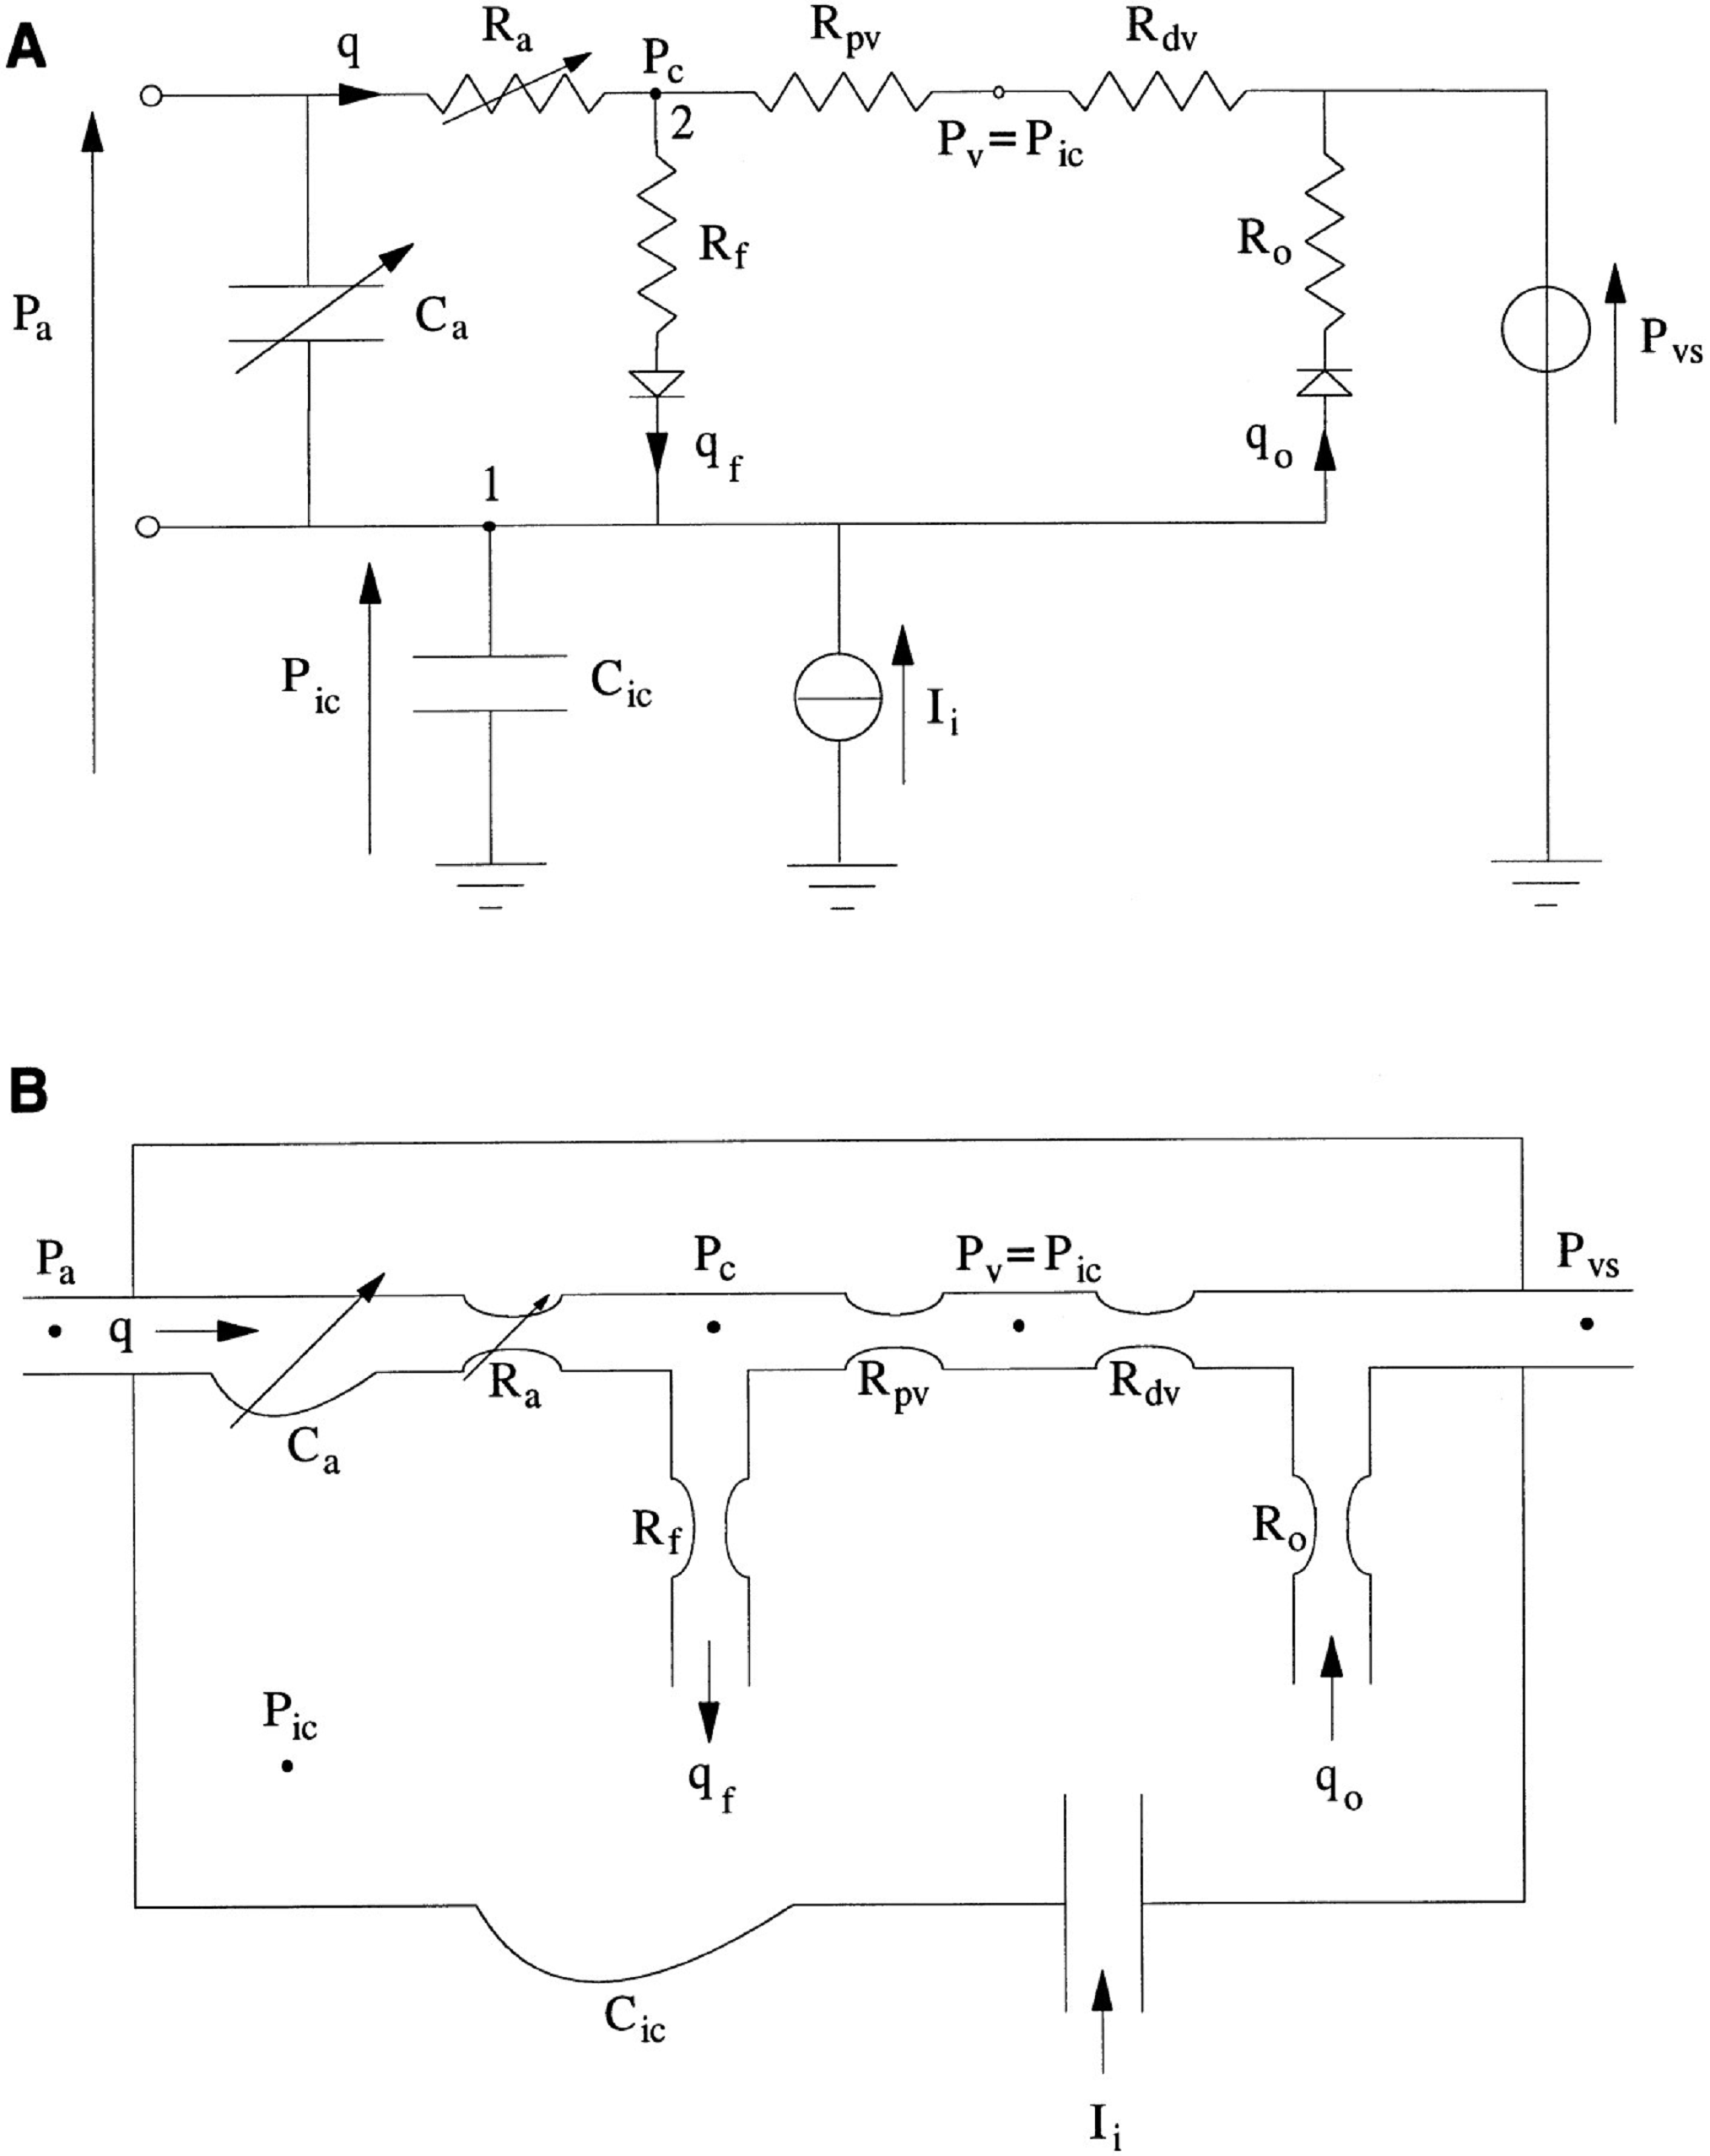
\includegraphics[width=12cm]{4_1_ursino}
\caption{Schéma du modèle d'Ursino (\cite{Ursino1997}).}
\label{fig:4_1_ursino}	
\end{figure}
Ce modèle permet de bien voir l'analogie électrique sur laquelle se base la partie linéaire de la
modélisation en compartiments. Les flux d'un compartiment à un autre sont reliés aux différences de
pression par des résistances hydrodynamiques :
\begin{equation}
F\,=\,R\,\Delta P.
\end{equation}
où $F$ est le flux en ml/min, $R$ la résistance en mmHg min/ml et $\Delta P$ la différence de pression en mmHg.
Les résistances elles-mêmes sont des paramètres du modèle, sans qu'une hypothèse de type loi de Poiseuille
par exemple les associe à des caractéristiques structurales des vaisseaux. De plus le caractère flexible
des parois, pouvant conduire à une accumulation de liquide dans un compartiment, est représenté par
une capacité C (en cm\^3/mmHg), elle non plus non reliée pour l'instant à un paramètre structural mesurable. Le volume
de chaque compartiment varie à la fois du fait du bilan des entrées et sorties de fluide, mais dépend
aussi des différences de pression entre sa pression intérieure et la pression intracrânienne via une compliance $C$:
\begin{equation}
V\,=\,C\,(P-P_{inc }).
\end{equation}
On aboutit à un ensemble clos d'équation différentielles soluble. Les paramètres sont alors estimés à
partir de valeurs moyennes venues de mesures disponibles dans la littérature, et en reproduisant des
données dynamiques typiques, telles qu'un flux hémodynamique moyen de 12.5 ml/s.\\
Le modèle de Sorek et al. (\cite{Sorek1988}) est plus complet: 7 compartiments (jugulaires et LCS en plus),
mais basé sur les mêmes hypothèses linéaires, et des équations semblables (figure ~\ref{fig:4_2_sorek}). 
%%%
\begin{figure}[!t]
\centering
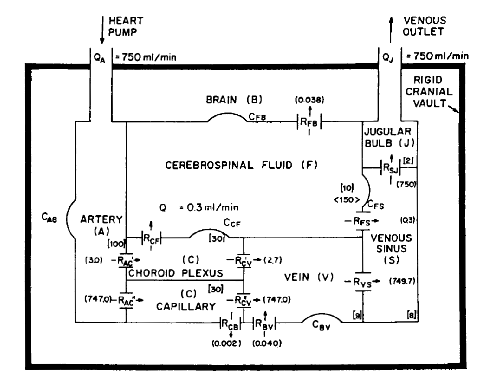
\includegraphics[width=12cm]{4_2_sorek}
\caption{Schéma du modèle de Sorek (\cite{Sorek1988}).}
\label{fig:4_2_sorek}	
\end{figure}
Les paramètres de
résistance et de compliance sont estimés à l'aide d'une procédure d'inversion linéaire à partir d'un jeu
de données de pression d'entrée en fonction du temps. Ils ne sont comme précédemment pas reliés à
des caractéristiques structurales.\\
Le modèle de Zagzoule et Marc-Vergnes (\cite{Zagzoule1986}) constitue la première approche basée sur des
données structurales mesurées (ou estimées), et de surcroît n'est plus linéaire. 

Le modèle n'est pas
stricto sensu compartimental, mais est présenté ici comme base du modèle de Linninger et al(\cite{Linninger2009}) , qui
reprend les mêmes idées dans une logique compartimentale. L'ensemble de la circulation
intracrânienne est représentée par une série de compartiments en parallèle et en série, selon un
schéma inspiré de la physiologie moyenne des artères, des veines, et des niveaux de microcirculation
intermédiaire. Le liquide cérébro-spinal et le parenchyme sont absents du modèle, si bien que rien ne
vient imposer la constance du volume intracrânien. Chaque compartiment est représenté par un tube,
et les paramètres du modèle sont les sections et les vitesses moyennes calculées en des points
discrétisés le long de chaque tube, la longueur du tube étant prise comme constante. Les équations de l'hydrodynamique sont transformées en ces points en équations aux différences finies (voir figure~\ref{fig:4_3_zagzoule}). 

Le système
d'équation est
\begin{eqnarray}
 \mbox{Continuité\hspace{1cm}}&&\frac{\partial A}{\partial t}\,+\,\frac{\partial A U}{\partial x}\,=\,0,\\
\mbox{Mouvement\hspace{1cm}}&&\frac{\partial U}{\partial t}\,+\,\frac{\partial}{\partial x} \biggl(\frac{U^2}{2}\,+\,\frac{P}{\rho}\biggr)\,=\,-F,\\
\mbox{\'Elasticité  des tubes\hspace{1cm}}&&E_L\biggl(\frac{A}{A_0}\,-\,1\biggr)\,=\,P,
\end{eqnarray}
où $U$ est la vitesse moyenne du flux sur l'aire $A$, $P$ la pression transmurale, $\rho$ la densité du fluide, $F$ le terme de friction, $E_L=\frac{E}{2}\frac{h}{R_0}$ avec $E$ le module Young, $h$ l'épaisseur de la paroie, $R_0$ et $A_0$ l'aire respectivement le rayon de la paroie et l'aire à une pression transmurale nulle.
 Ceci constitue un système hyperbolique du premier ordre complet. 
%%%
\begin{figure}[!t]
\centering
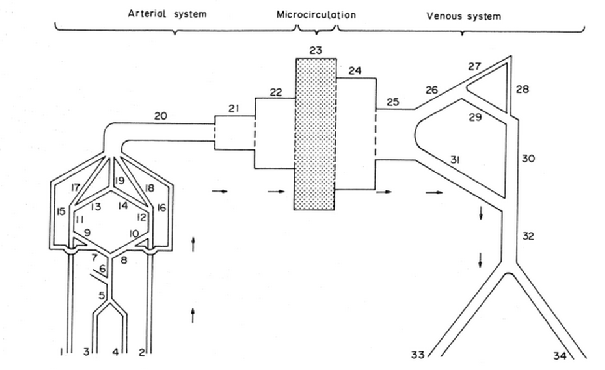
\includegraphics[width=14cm]{4_3_zagzoule}
\caption{Schéma du modèle de Zagzoule et Marc-Vergnes (\cite{Zagzoule1986}).}
\label{fig:4_3_zagzoule}	
\end{figure}


Une équation constitutive
supplémentaire relie la friction et les vitesses, selon une loi de Poiseuille :
\begin{equation}
\label{eq:poiseuille}
F\,=\,N\biggl(\frac{8\,\pi\,\mu}{\rho}\frac{U}{S}\biggr).
\end{equation}
où $\mu$ est le coefficient de viscosité dynamique, $S$ l'aire totale ($S = NA$, $N$ étant le nombre de vaisseaux). Cette loi de Poiseuille permet d'associer au modèle les paramètres structuraux des vaisseaux, soit tirés
de la littérature, soit estimés. Par exemple, les paramètres de diamètre et de nombre des capillaires
dans la partie microcirculatoire sont estimés sur la base d'une progression géométrique en l'absence
de données. L'ensemble fournit des valeurs de pression et de flux dans le système circulant
comparables aux valeurs mesurées, et précède une étude simplifiée de mécanismes possibles
d'autorégulation.\\
Présentons pour finir le modèle de Linninger et al. (\cite{Linninger2009}), qui est le plus proche dans l'esprit du
nôtre. L'objectif clinique de ce modèle est la modélisation de pathologies du liquide cérébro-spinal,
telles que l'hydrocéphalie. Dans ce but, il propose une description plus détaillée de la circulation du
LCS. Les quatre ventricules sont séparés en compartiments distincts. Cette logique le conduit alors à
une latéralisation de la description du système sanguin, afin d'associer chaque ventricule latéral à son
propre système artériolaire (lieu de la production du LCS). Enfin, il incorpore un comportement
parenchymateux également latéral. Le tout est englobé dans un compartiment sous-arachnoïdien
commun, qui se déverse dans le canal de la moelle épinière (voir Figure~\ref{fig:4_4_linninger}). 

Dans la description de
chaque compartiment, il reprend les variables géométriques du modèle précédent : aire et flux
entrants et sortants, mais sans discrétiser le long des tubes une équation aux dérivées partielles, ce
qui n'aurait guère de sens pour les compartiments du LCS, pour lesquels cette géométrie est peu
physiologique de toute façon. On revient à des équations bilan pour la quantité de mouvement et la
masse. Notons toutefois qu'ici la résistance hydrodynamique n'est plus modélisée entre les
compartiments, mais à l'intérieur de ceux-ci, via une loi de Poiseuille globale le long des tubes. Par
ailleurs la capacité des compartiments à jouer leur rôle « capacitif » est représentée par une équation
de distensibilité
\begin{equation}
P\,-\,P_{Brain}\,=\,E\biggl(\frac{A}{A_0}\,-\,1\biggr).
\end{equation}
où $P_{brain}$ est la pression dans le parenchyme. et $E$ l'élastance. On complète le système par des équations assurant la continuité des flux d'un compartiment à
l'autre. La contrainte de Monro-Kellie est implémentée, contrairement au modèle de Zagzoule. Les
données fournies au modèle pour l'intégrer sont le décours temporel de la pression en entrée (artère
carotide) et en sortie (veine jugulaire). Le modèle permet alors de calculer tous les flux et les pressions
au cours du temps dans tous les compartiments. Il reproduit de façon assez détaillée des données
pathologique dynamiques sur l'hydrocéphalie.\\
%%%
\begin{figure}[!t]
\centering
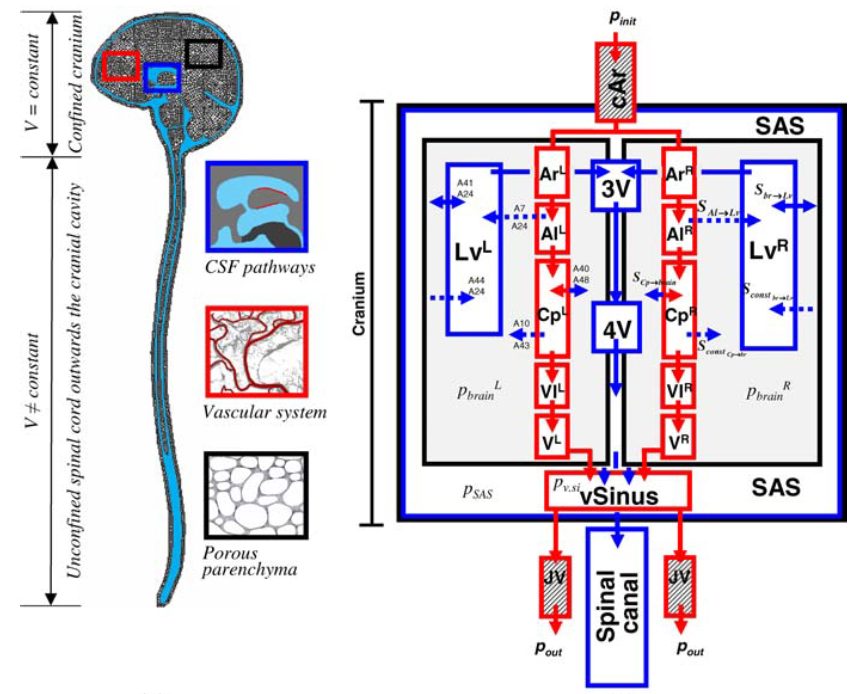
\includegraphics[width=12cm]{4_4_linninger}
\caption{Schéma du modèle de Linninger (\cite{Linninger2009}).}
\label{fig:4_4_linninger}	
\end{figure}
Ce modèle constitue un intéressant compromis entre d'une part la logique de compartiments,
et d'autre part l'introduction de paramètres structuraux et physiologiques mesurables
indépendamment du modèle. Néanmoins, malgré la relative complexité du modèle (86 équations
algébro-différentielles non-linéaires couplées pour 22 compartiments), il correspond encore à une
modélisation « moyenne » des écoulements, et ne s'adapte pas à des données obtenues sur un
individu particulier.\\
Notre démarche a été donc de s'inspirer de l'approche de Zagzoule et Linninger, mais en allant
beaucoup plus loin dans l'introduction de paramètres anatomiques issus de l'imagerie d'un patient
donné. En effet, indépendamment de l'approche en compartiments développée dans cette partie,
plusieurs travaux ont commencé à proposer des approches de modélisation patient-spécifique.
Exposons-les brièvement.
%%%
%%%
%%%
\section{Intégration de données structurales}
La variabilité de la structure vasculaire cérébrale, en particulier des anastomoses artérielles et
veineuses, l'importance pathologique de cette variabilité, ont conduit à la nécessité de proposer des
approches de modélisation permettant de comprendre la portée physiologique de ces variantes
structurales. C'est la structure artérielle, en particulier le polygone de Willis, qui a fait l'objet des
recherches les plus nombreuses. On suivra ici le bilan de ces travaux donné dans (\cite{David2008}).\\
L'article de Cebral et al. (\cite{Cebral2003}) utilise des données d'imagerie par temps de vol du cercle de Willis
et des principales artères pour générer une structure 3D détaillée, considérée comme un système de
parois rigides, et maillée spatialement. Les données dynamiques d'entrée sont fournies par une
mesure des flux en contraste de phase. Une résistance effective à la sortie du système est proposée
par différentes techniques de modélisation de la perfusion aval, permettant de calculer une pression
de sortie, et de rendre ainsi le modèle soluble en 3D plus temps. La solution met en évidence des
écoulements non stationnaires, et se concentre en particulier sur le problème du rôle régulateur du
cercle de Willis lors de l'occlusion d'une carotide.\\
Le travail de Kim et al. (\cite{Kim2006}) ajoute à cette approche l'extensibilité des parois du système
artériel, et se base sur le même type de données structurales issues de l'imagerie par temps de vol.
Les conditions aux limites en entrée sont ici les pressions afférentes et non les flux. Les pressions en
sortie sont à nouveau calculées sur la base de modèles de résistances idéalisées du réseau perfusant
en aval. Noter qu'un modèle simple d'autorégulation est proposé. Le modèle se concentre sur la
prédiction de la réponse des anastomoses du cercle de Willis lors d'un épisode de réduction abrupte
de la pression dans une artère d'entrée.\\
Enfin Moore et al. (\cite{Moore2006}) ont suivi pour l'essentiel les mêmes stratégies, se distinguant par une
modélisation différente du réseau aval. Il est à noter en effet que la description simplifiée de
l'architecture aval constitue la partie la moins solide de ces modélisations, en contraste avec la vision
très détaillée du système artériel. Notre approche de ce point de vue cherche à combiner une
description globale issue des données les plus avancées disponibles, y compris sur la géométrie du
cercle de Willis, avec la vision la plus simple possible des compartiments individuels. Nous pourrons
ainsi, comme nous l'exposions dans l'introduction, adapter le plus étroitement la finesse de description
du modèle avec celle des données, pour l'ensemble de la circulation cérébrale.
%%%
%%%
%%%
\section{Vers un modèle complet sujet-spécifique}
%%%
%%%
\subsection{Exposition du modèle}
L’anatomie vasculaire du cerveau est complexe. Un grand nombre de vaisseaux assurent
l’apport du sang dans les différentes régions cérébrales. Il est difficile d’accéder aux caractéristiques de l’ensemble du système, et de le modéliser directement. Beaucoup de travaux se focalisent alors sur
des structures locales précises comme le polygone de Willis ou tentent de simplifier le problème en
regroupant les vaisseaux par type afin de travailler avec moins de compartiments (voir~\ref{sec:modeles_compartiments}). Jusqu’à
présent, la plupart des modèles vasculaires intégrant des données d’imagerie se contentaient du
versant artériel de la circulation en des données de contraste de phase et/ou d’une imagerie par temps
de vol. L’avancée des séquences IRM permet à présent d’accéder à un grand nombre d’informations
sur les flux intracrâniens, tant au niveau anatomique, que dynamique et physiologique. En parallèle,
les outils informatiques autorisent la simulation de problèmes complexes intégrant de nombreux
compartiments.\\
Dans ce contexte la modélisation d’un système complet des flux dans le cerveau avec
architecture réaliste et adaptée au sujet devient envisageable. Notre objectif, comme nous l’avons
déjà dit, est de développer une méthodologie permettant pour un sujet donné, d’extraire son
arborescence vasculaire ainsi qu’un maximum d’informations permettant de caractériser les flux
intracrânien afin de nourrir le modèle. C’est ce qui a été réalisé dans les chapitres précédents.\\
Le modèle tel que nous le proposons maintenant se base sur les mêmes principes que les
travaux de Zagzoule et Marc-Vergnes (\cite{Zagzoule1986}) , puis de Linninger et al. (\cite{Linninger2005},~\cite{Linninger2007},~\cite{Linninger2009}) qui intègrent comme
nous l’avons vu les compartiments vasculaires et céphalo-rachidien sous forme de tubes. Dans une
logique de simplification, leur modèle ne considère qu’une entrée, fusion des différentes carotides
internes et de l’artère basilaire, puis un système de tubes simples allant des artères aux veines (1 par
type et par hémisphère), enfin une sortie pour le sang, fusion des veines jugulaires, et une voie de
sortie pour le liquide céphalo rachidien, la moelle épinière.\\
Dans le chapitre 3 nous avons mis au point une chaine de traitement qui aboutit à une
architecture complète partant des carotides internes et de l’artère basilaire, et allant jusqu’aux veines
jugulaires. Comme tous les travaux de modélisation antérieurs, nous n’avons pas accès aux
compartiments artériolaires, capillaires et veinulaires ; nous avons donc des « super tubes »
regroupant en réalité un grand nombre de vaisseaux. La différence de notre travail avec celui par
exemple de Linninger, réside dans le nombre de de ces structures. Pour chaque artère terminale que
nous pouvons identifier, nous retrouverons un ensemble artériole, capillaire, veinule définissant un
territoire.\\
Du côté de la sortie, le système veineux se termine par les sinus puis les veines jugulaires.
Quelques simplifications sont également possibles à ce niveau. L’une des caractéristiques distinguant
certains sinus est en effet leur capacité à réabsorber une partie du liquide céphalo rachidien via les
villosités arachnoïdiennes. Ce transport est prépondérant dans le sinus sagittal supérieur (voir~\ref{sec:syst_ventr}). Afin de limiter la complexité du modèle, nous faisons le choix de regrouper les sinus veineux autres
que le sinus sagittal supérieur en un « super sinus » représentant la sortie de notre système. On peut
alors représenter la nouvelle architecture comme suit (Figure~\ref{fig:4_5_schema_modele}):
%%%
\begin{figure}[!t]
\centering
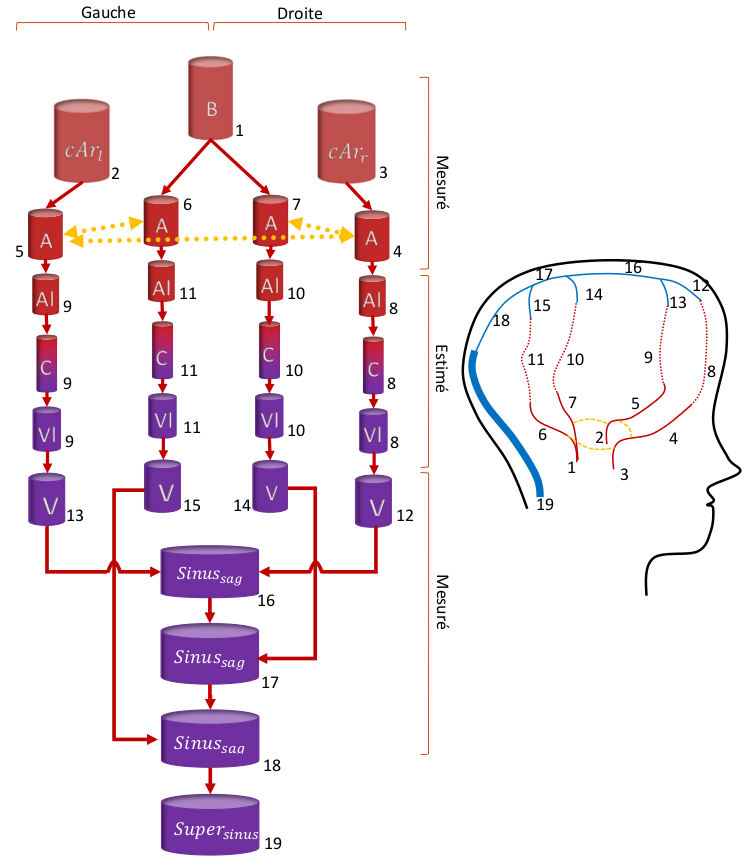
\includegraphics[width=12cm]{4_5_schema_modele}
\caption{Illustration de la circulation sanguine pour le modèle développé. Dans cet exemple, afin d’améliorer la lisibilité,
nous considérons un système circulatoire sans artères cérébrales moyennes et avec très peu de ramifications. A gauche est
représenté la structure sous forme de tubes. Avec $B$ pour artère basilaire, $Car$ pour carotide interne, $A$ pour artère, $A_l $pour
artériole, $C$ pour capillaire, $V_l $pour veinule, $V$ pour veine, et $Sinus_{sag}$ pour sinus sagittal supérieur. Les flèches en pointillés
orange indiquent la présence de liens entre ces artères (communicantes). Le schéma de droite illustre la structure
anatomique correspondant au graphe de gauche, les numéros font le lien entre les segments du schéma et le tubes du
graphe.
}
\label{fig:4_5_schema_modele}	
\end{figure}
Cette structure est à mettre en relation avec le modèle de Linninger (Figure~\ref{fig:4_4_linninger}). Nous n’avons
cependant ici représenté que le système sanguin, le système céphalo-rachidien étant identique aux
travaux de ce dernier (Figure~\ref{fig:4_4_linninger}) à la subtilité près que les interactions LCS – Parenchyme – Sang sont
réparties sur un ensemble de tubes (plusieurs artérioles et capillaires).\\
Le sang est modélisé comme un fluide visqueux et incompressible évoluant des artères aux veines
(Figure~\ref{fig:4_5_schema_modele}). Le système céphalo-rachidien intègre les ventricules latéraux, les troisième et quatrième
ventricules et l’espace sous arachnoïdien (cérébral et de la moelle), le tout étant interconnecté (Figure~\ref{fig:4_6_LCR_modele}). A partir de l’espace sous arachnoïdien cérébral, on admet que le LCS est réabsorbé dans le sinus
veineux par l’intermédiaire des villosités arachnoïdiennes (\cite{Segal2001}). Le parenchyme est considéré comme
un milieu déformable et incompressible séparé en deux hémisphères et composé de deux phases : le
fluide extracellulaire (30\% du parenchyme, similaire au liquide cérébro-spinal) et la matrice cellulaire
solide (70\% du parenchyme) représentant les neurones, les cellules gliales et les fibres axonales. De
tous les compartiments, seule la moelle épinière n’est pas contenue dans le crâne. Enfin, il existe des
entrées additionnelles au modèle, autre que les trois artères principales, à savoir : la production constante de liquide cérébro-spinal depuis les artérioles vers les ventricules latéraux par les plexus
choroïdes et la production diffuse des capillaires vers le parenchyme cérébral puis les ventricules.\\
%%%
\begin{figure}[!t]
\centering
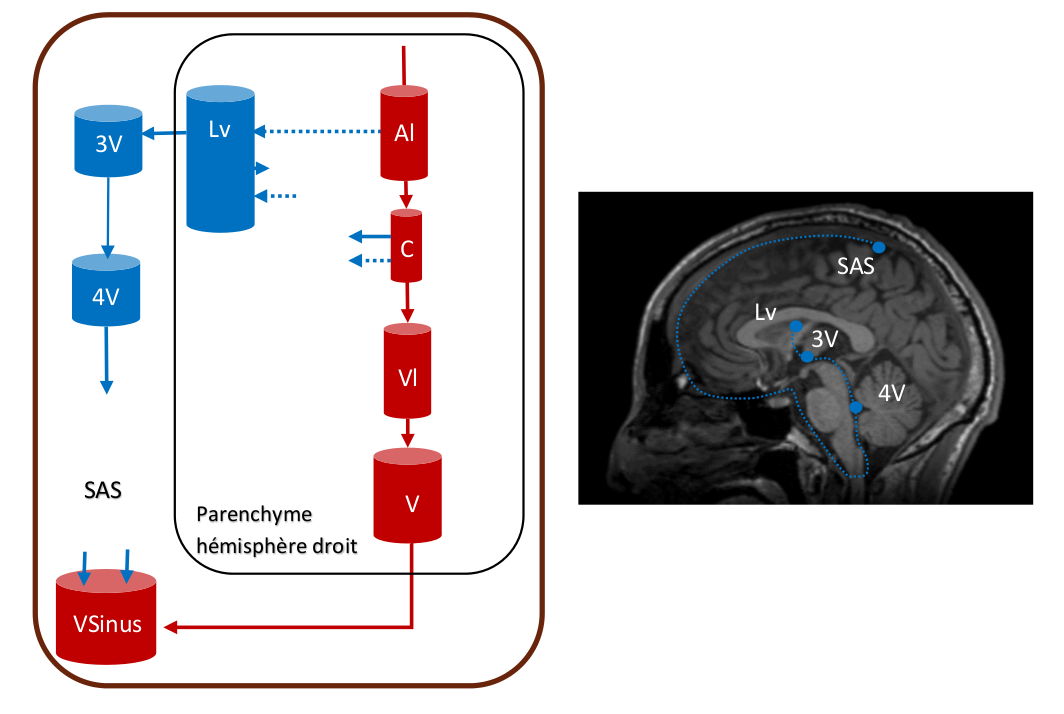
\includegraphics[width=12cm]{4_6_LCR_modele}
\caption{Système cérébro-spinal dans notre modèle en prenant une référence partant d’une artériole. En rouge sont
indiqués les flux sanguin, en bleu les flux du LCS. Les flèches en pointillés indiquent la production de LCS (constante), tandis
que les flèches pleines représentent les échanges de liquide liés à la pression. $L_v$ représente les ventricules latéraux, $3V$ le
troisième ventricule, $4V$ le quatrième ventricule, $SAS$ l’espace sous arachnoïdien, $VSinus$ le sinus veineux. L’image de droite
illustre l’évolution du liquide cérébro-spinal (ligne en pointillé), les points représentant les compartiments.}
\label{fig:4_6_LCR_modele}	
\end{figure}
La doctrine de Monroe-Kellie est rigoureusement implémentée dans le modèle. Cependant le
liquide cérébro-spinal peut s’écouler dans l’espace sous arachnoïdien de la moelle qui n’est pas confiné
dans crâne.\\
Le flux sanguin et cérébro-spinal est décrit dans ce modèle par les équations bilans fondamentales
de l’hydrodynamique : conservation de la masse, conservation de la quantité de mouvement. Pour
tenir compte de l’adaptation du diamètre des vaisseaux aux pressions on introduit pour chaque
compartiment un paramètre d’élasticité de la paroi et une équation correspondante. Le modèle
contient trois type de variables pour chaque compartiment : la pression au centre $p$, le flux entrant fin
et sortant $f_{out}$ et l’aire du tube $A$. Le principe est d’avoir un système d’équations générique pour un
tube que l’on peut ensuite reproduire pour un nombre indéfini de tubes, à condition de s’assurer de
règles de continuité adéquate entre compartiments.\\
Notons que, contrairement à Linninger, nous représentons les pressions au centre du tube et non
en fin de tube (Figure~\ref{fig:4_7_milieu_tubes}).\\
%%%
\begin{figure}[!t]
\centering
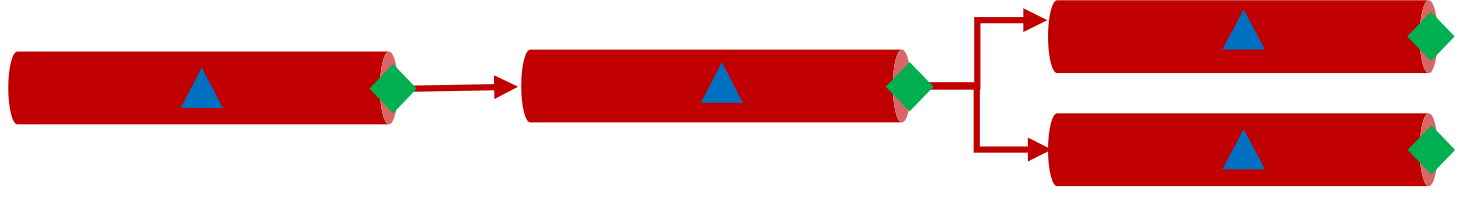
\includegraphics[width=12cm]{4_7_milieu_tubes}
\caption{Différence entre la définition des pressions sur le modèle de Linninger, et sur le nôtre. Les triangles bleus
indiquent les pressions selon notre modèle et les losanges verts selon Linninger.}
\label{fig:4_7_milieu_tubes}	
\end{figure}
La conservation de la masse assure qu’aucun volume de fluide n’est gagné ni perdu,
conformément à l’hypothèse d’incompressibilité du sang et du LCS. On peut ainsi écrire cette équation
sous la forme :
\begin{equation}
l\,\biggr(\frac{\partial A}{\partial t}\biggr)\,=\,f_{in}\,-\,f_{out}\,+\,S_{I\rightarrow II}.
\end{equation}
avec $l$ la longueur hydraulique du compartiment, $\frac{\partial A}{\partial t}$
le changement de l’aire de la section du tube en
fonction du temps, et $f_{in}$ et $f_{out}$ les débits en entrée et en sortie. $S_{I \rightarrow II}$ est dans ce bilan un terme de
source reflétant le transfert (constant ou non) d’un compartiment à un autre. Ce terme ne sera
pertinent que pour les compartiments disposant de parois perméables autorisant le transfert avec une autre phase. Pour commencer, la production du LCS est principalement lié à un transfert constant
entre le compartiment artériolaire et les ventricules latéraux $S_{Al\rightarrow Vl}$. Cependant, une seconde
production existe à travers les capillaires qui produisent de façon constante du LCS passant dans
l’espace extracellulaire du parenchyme ce qui conduit à un terme $S^{const}_{Cp\rightarrow cerv}$. Cette production peut
ensuite rentrer dans les ventricules du fait de la différence de pression via une résistance
hydrodynamique :
\begin{equation}
P_{Lv}\,-\,P_{cerv}\,=\,\alpha\,S_{cerv\rightarrow Lv},
\end{equation}
à laquelle s’ajoutera un transfert constant $S^{const}_{cerv\rightarrow cLv}$. Enfin il peut exister une fuite du lit capillaire
vers le parenchyme dans les deux sens $S_{Cp\rightarrow cerv}$ , du fait de la différence de pression entre les capillaires
et le cerveau environnant (\cite{Starling1896}). La résorption du LCS par le sinus veineux est principalement réalisée
au niveau des villosités arachnoïdiennes. Cette résorption est elle aussi modélisée comme fonction de
la différence de pression entre l’espace sous arachnoïdien et le sinus veineux et d’une constante $k$, on
définit ainsi $f_{reabsorption}$ :
\begin{equation}
f_{reabsorption}\,=\,k\,(P_{SAS}\,-\,P_{sinusV}),
\end{equation}
avec $P_{SAS}$ la pression dans l’espace sous arachnoïdien, $P_{sinusV}$ la pression dans le sinus veineux, et $k$
le coefficient de réabsorption.
L’équation de conservation de la quantité de mouvement permet de relier la chute de pression
$\Delta P$ au débit sanguin $f_{in}$ . Nous utilisons une équation similaire à la loi d’Hagen-Poiseuille :
\begin{equation}
\label{eq:flux}
P_{in}\,-\,P\,=\,\Delta P\,=\,\biggl(\frac{a_{in}}{2}\,+\,,\frac{a}{2}\biggr)\,f_{in},
\end{equation}
où $P_{in}$ in est la pression du compartiment précédent, et $P$ la pression dans le compartiment courant. Le
terme $a=\frac{8\pi \mu l}{A^2}$ est un terme de résistance à l’écoulement qui tient compte de la chute de pression le long du
compartiment du fait des forces visqueuses ; il dépend de la viscosité dynamique du fluide, $\mu$, de la
longueur hydraulique du compartiment, $l$, et inversement du carré de l’aire de la section du compartiment. Pour un
vaisseau plus étroit la résistance augmente et une chute de pression plus importante sera nécessaire
afin de maintenir le même flux. Cette approche est similaire à l’Équation~\ref{eq:poiseuille}. Dans notre modèle, $a$
peut être calculé directement depuis les données morphologiques recueillies (voir chapitre~\ref{chap:imageriemorpho}) pour
certains compartiments mais doit être estimé sur la base de la littérature pour les artérioles, les
capillaires et les veinules. Comme vu dans la partie~\ref{sec:finalisation} nous avons contraint le système pour n’avoir
que des jointures en Y entre les tubes (deux tubes vers un ou l’inverse).\\
Dans ces situations la formule doit légèrement s’adapter :
\begin{equation}
\label{eq:ley}
\frac{a_{in_1}}{2}\,(P\,-\,P_{in_2})\,+\,\frac{a_{in_2}}{2}\,(P\,-\,P_{in_1})\,=\,\biggl(\frac{a_{in_1}}{2}\,\frac{a_{in_2}}{2}+\frac{a_{in_1}}{2}\,\frac{a}{2}+\frac{a_{in_2}}{2}\,\frac{a}{2}\biggr)\,f_{in},
\end{equation}
avec $a_{in_1}$ , $a_{in_2}$ , $P_{in_1}$ et $P_{in_2}$ les paramètres des deux parents du tube courant (voir Figure~\ref{fig:4_8_param_tubes} et Annexe~\ref{sec:deriveq}).\\
%%
\begin{figure}[!t]
\centering
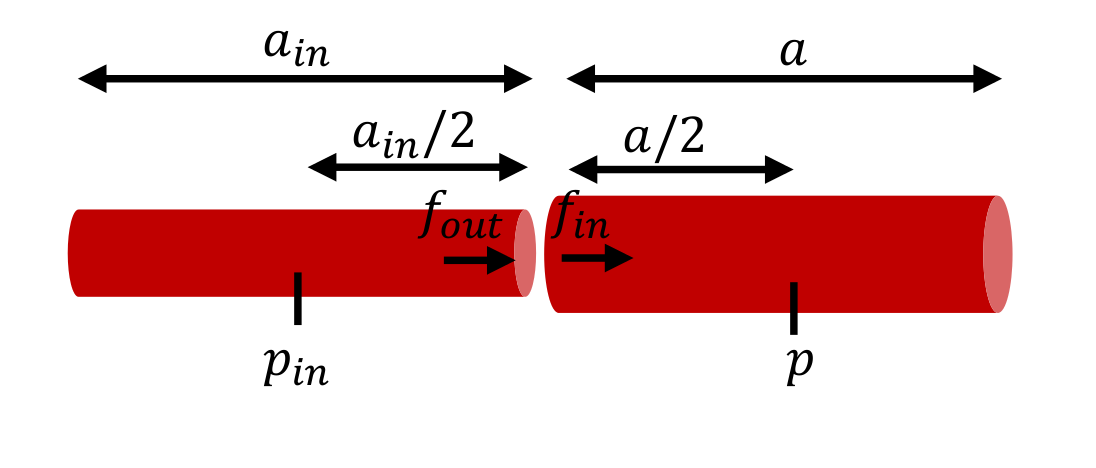
\includegraphics[width=12cm]{4_8_param_tubes}
\caption{Illustration des différents paramètres des tubes et de leur positionnement lorsque deux tubes se suivent.}
\label{fig:4_8_param_tubes}	
\end{figure}

Des équations additionnelles connectant les compartiments ont ensuite été définies selon :
\begin{equation}
P \,-\,P_{next}\,=\,\Delta\,P\,=\,\biggl(\frac{a}{2}\,+\,\frac{a_{next}}{2}\biggr)\,f_{out},
\end{equation}
avec $P_{next}$ la pression dans le tube fils et $a_{next}$ la résistance de ce tube. $f_{out}$ est le flux sortant du
tube. Dans le cas d’une connexion en Y, l’équation devient :
\begin{equation}
\frac{a_{next_1}}{2}\,(P\,-\,P_{next_2})\,+\,\frac{a_{next_2}}{2}\,(P\,-\,P_{next_1})\,=\,\biggl(\frac{a_{next_1}}{2}\,\frac{a_{next_2}}{2}+\frac{a_{next_1}}{2}\,\frac{a}{2}+\frac{a_{next_2}}{2}\,\frac{a}{2}\biggr)\,f_{out}.
\end{equation}
On garantit implicitement grâce à cette équation et l’Équation~\ref{eq:flux}, que le fluide n’est jamais perdu
entre la sortie d’un vaisseau et l’entrée du vaisseau suivant ($f_{out}^{parent}\, = \, f_{in}^{fils}$ ).\\
Comme on l’a dit on doit par ailleurs décrire l’élasticité de chaque compartiment par une
équation associée. Les compartiments ont en effet différents degrés d’élasticité. Les artères qui
entourent le cerveau sont moins rigides que les vaisseaux profondément intégrés dans le tissu
cérébral. Il s’agit d’un rôle de type « capacitif » pour les compartiments, dans l’analogie d’un circuit
électrique, qui leur permet de stocker temporairement un volume sanguin. On le représente par une
équation passive classique dans la littérature  (\cite{Zagzoule1986},~\cite{Linninger2009}) qui ne prend pas en compte à ce stade les
phénomènes d’autorégulation (\cite{Paulson1990}) :
\begin{equation}
P_{lumen}\,-\,P_{cerv}\,=\,E\,\biggl(\frac{A}{A_0}\,-\,1\biggr).
\end{equation}
L’écart à la section de repos du vaisseau $A-A_0 $est gouverné par l’élastance du vaisseau $E$ et la
différence de pression entre la lumière du vaisseau et le parenchyme $P_{lumen}\,-\,P_{cerv}$ . $A_0$
représente l’aire de la section à une pression transmurale nulle. Ainsi, plus la pression transmurale
sera grande, plus le vaisseaux se contractera ou se dilatera. De même, lorsque la pression sanguine
dépasse la pression intracrânienne du tissu cérébral environnant, le vaisseau se dilate, et inversement
lorsque la pression est plus faible. Cette approche permet de coupler les équations de flux sanguines
et cérébro-spinales avec la pression du parenchyme en prenant en compte l’élasticité du vaisseau.\\
Un système de 4 équations génériques pour le système sanguin et cérébro-spinal est donc
défini et pourra être généré automatiquement pour l’ensemble de l’architecture.\\
Afin de garantir la constance du volume de la doctrine de Monro-Kellie une équation doit être
rajoutée pour laquelle nous suivons Linninger (\cite{Linninger2009}):
\begin{equation}
V_{TotalCervHem}\,=\,\sum_b V_b\,+\,\sum_{LCR} V_{LCR}\,+\, V_{CervHem}\,=\,constante,
\end{equation}
ou encore :
\begin{equation}
\bigl(V_{Ar}^{L,R}\,+\,V_{Al}^{L,R}\,+\,V_{Cp}^{L,R}\,+\,V_{Vl}^{L,R}\,+\,V_{V}^{L,R}\,+\,V_{sSin}^{L,R}\bigr)\,+\,\bigl(V_{Lv}^{L,R}\,+\,0.5\,V_{3V}\,+\,0.5\,V_{4V}\,+\,V_{SAS}\bigr)\,=\,constante
\end{equation}
où on a :
\begin{equation}
V_{CervHem}\,=\,V_{exfCerv}^{L,R}\,+\,V_{solidCerv}^{L,R}\,=\,A_{exfCerv}^{L,R} l_{exfCerv}^{L,R}\,+\,A_{solidCerv}^{L,R} l_{solidCerv}^{L,R},
\end{equation}
et {\em exfCerv} correspond au fluide extracellulaire dans les deux hémisphères, {\em solidCerv} à la matrice
cellulaire solide, $V$ la somme des volumes pour chaque compartiment.\\
\afterpage{%
    \clearpage% Flush earlier floats (otherwise order might not be correct)
    %\thispagestyle{empty}
	\begin{landscape}
	\begin {table}
	\captionof{table}{Tableau résumant les données utilisées dans les différents modèles de type compartiments de la littérature.} 
	\label{tab:modeles} 
	\centering
	\begin{tabularx}{\linewidth}{  |X | l | l |X | X | X | X | X | X | }
\hline
	 & Ursino et al. & Sorek et al. & Cebral et al. & Kim et al. & Moore et al. & Zagzoule et al. & Linninger et al. & Notre modèle \\
\hline
	Parenchyme & Oui & Oui & Non & Non & Non & Oui  & Oui & Oui  \\ 
	Artères & Oui & Oui & Oui & Oui & Oui & Oui & Oui & Oui \\ 
	Artérioles & Non & Non & Non & Non & Non & Oui  & Oui  & Oui  \\ 
	Capillaires & Oui & Oui & Non & Non & Non & Oui  & Oui  & Oui  \\ 
	Veinules & Non & Non & Non & Non & Non & Oui  & Oui  & Oui  \\ 
	Veines & Oui & Oui & Non & Non & Non & Oui  & Oui  & Oui  \\ 
	Sinus & Oui & Oui & Non & Non & Non & Oui  & Oui  & Oui \\ 
	LCS & Non & Oui & Non & Non & Non & Non  & Oui  & Oui  \\ 
\hline
	Données structurales & Théoriques & Théoriques & Mesurées & Mesurées & Mesurées & Mesurées et Théoriques & Mesurées et Théoriques + Pression en entrée mesurées & Mesurées et estimées \\ 
\hline
	Particularité& - & - & Architecture détaillée du polygone de Willis & Extensibilité des parois&  Se termine par un bloc poreux &  Intègre le polygone de Willis & Intègre le LCS et sépare le système en deux hémisphères& Se base sur les données structurales \\ 
\hline
	\end{tabularx}
	\end{table}
	\end{landscape}
\clearpage% Flush page
}
Le résumé des différents modèles est illustré dans le Tableau~\ref{tab:modeles}. Chaque modèle dispose de ces caractéristiques et prend en compte plus ou moins de compartiment. Nous tentons à travers notre modèle, de fournir la description la plus complète possible au vue des données d'imagerie IRM.






%%%
%%%
\subsection{Implémentation}
Les données morphologiques fournissent une structure sous forme de graphe contenant
l’ensemble des caractéristiques de l’arborescence. Ce graphe est construit sous MATLAB. Pour
implémenter sur la base de ce graphe le modèle décrit plus haut, nous avons fait le choix d’utiliser Java
et de proposer une interface graphique qui permet une meilleure fluidité et simplicité pour l’utilisateur
final. L’interface doit charger le graphe, proposer à l’utilisateur la possibilité d’ajuster les paramètres
tube par tube, rajouter ou supprimer des tubes. Une fois ces choix fait, on pourra générer le système
d’équations différentielles ordinaires à résoudre, au format MATLAB, et lancer la simulation, avant de
rapatrier les résultats (Figure~\ref{fig:4_9_implem}) et de les visualiser toujours dans la même interface.\\

Lors de la segmentation, le code MATLAB permettant de générer le graphe a produit un fichier texte
de format fixe contenant la définition de toutes les structures et les liens existants entre elles. Le fichier
prend une forme générique. Une première section définit les tubes, leur type (artère, veines etc.) et
leur caractéristiques morphologiques (aire, longueur etc.), tandis qu’une seconde informe sur la
structure de liens existants entre ces tubes. Ci-dessous un exemple de structur de fichier généré après la reconstruction du graphe. Notons que pour les débits, pressions et aire elles
servent de valeurs initiales.

\vspace{0.4cm}
{\tt \$TUBES \textcolor{green}{\% définitions des tubes}}

{\tt \textcolor{green}{\% [TypeTube\_ID]==TypeTube\_longueurID\_ID:valeur@@TypeTube\_alphaID\_ID:formule
@@TypeTube\_elastanceID\_ID:valeur@@TypeTube\_AireID\_ID:valeur@@TypeTu
be\_DebitEntrantID\_ID:valeur@@TypeTube\_DebitSortantID\_ID:valeur@@TypeTube\_Pr
essionID\_ID:valeur}}

{\tt \$LINKS \textcolor{green}{\% définition des liens A vers B donne A --> B}}

{\tt \textcolor{green}{\% [TypeTube\_ID]—-> [TypeTube\_ID]}}

{\tt [TI\_1]--> [R\_T0\_20]}

{\tt [R\_T0\_20]--> [R\_T0\_3]}

\vspace{0.4cm}
%%%
\begin{figure}[!b]
\centering
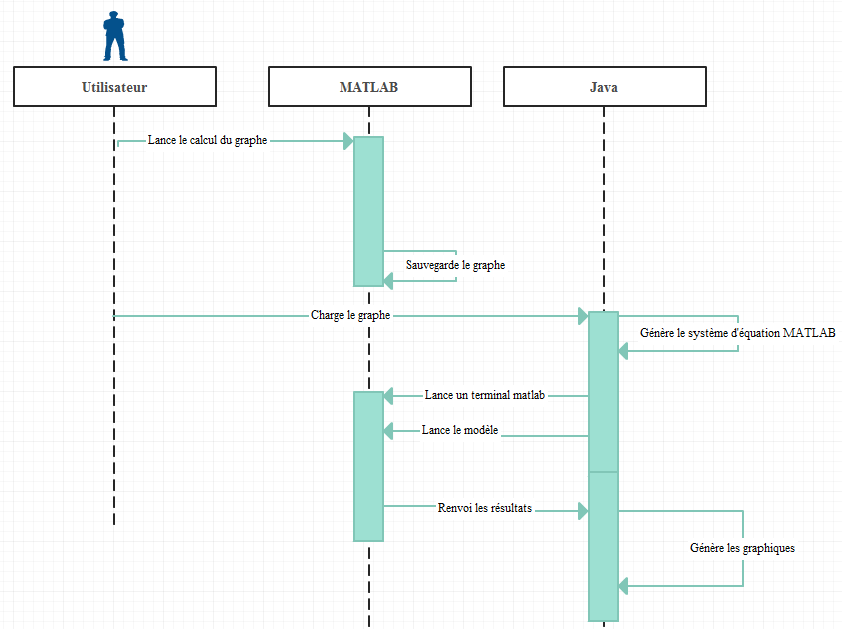
\includegraphics[width=12cm]{4_9_implem}
\caption{Diagramme de séquence général de la chaine de traitement du modèle. Dans une première partie les données
morphologiques permettent de générer le graphe sous MATLAB, ce graphe est sauvegardé en vue d’être chargé par
l’utilisateur dans un logiciel Java qui permettra de générer le système d’équations correspondant, lancer le terminal MATLAB
et le modèle pour enfin récupérer les résultats.}
\label{fig:4_9_implem}	
\end{figure}
Ce fichier est celui qui sera chargé dans l’interface Java de façon à générer une représentation
graphique sous forme de blocs modulaires et modifiables. Cet outil peut être aussi utilisé pour définir
des architectures complètement arbitraires (Figure~\ref{fig:4_10_interface_java}). La structure de liens et les caractéristiques des
tubes peuvent à ce stade être modifiées par l’utilisateur.\\
%%%
\begin{figure}[!t]
\centering
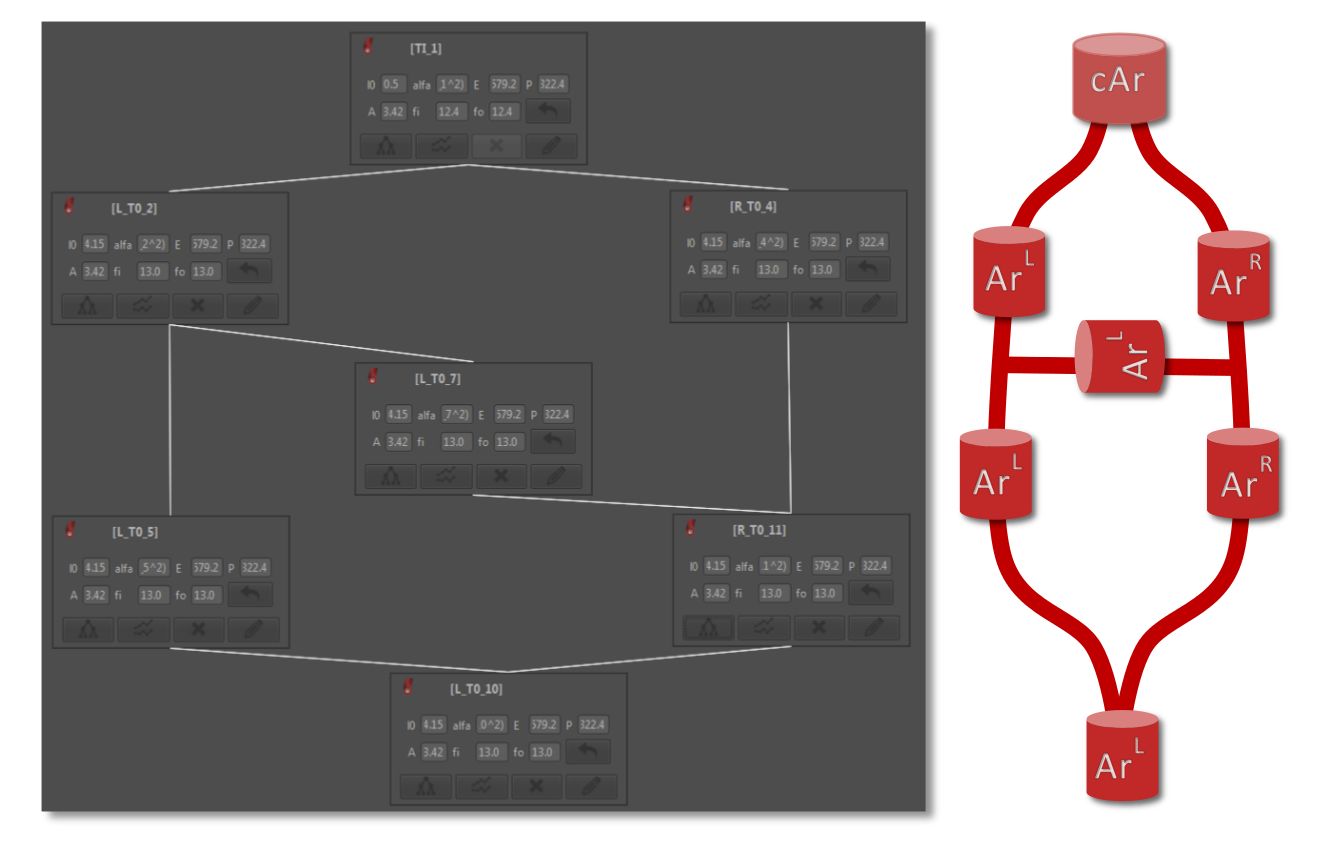
\includegraphics[width=12cm]{4_10_interface_java}
\caption{Exemple de structure affichée dans l'interface Java pour une architecture arbitraire. La structure arbitraire prise
en référence est indiquée par le schéma à droite.}
\label{fig:4_10_interface_java}	
\end{figure}
Une fois la structure validée, l’utilisateur lance la simulation. Le programme valide alors
l’architecture afin de s’assurer qu’il n’y ait pas d’incohérences (par exemple un tube à la fois parent et
fils d’un autre), et créé le système d’équations qu’il écrit dans trois fichiers MATLAB. Le premier
contient le programme principal avec définition des variables initiales (pressions d’entrées etc.) et la
boucle d’itérations du modèle au cours du temps. Les deux autres fichiers contiennent les équations à
résoudre sous une forme discrétisées par une méthode d’Euler explicite. Le logiciel lance ensuite un
terminal MATLAB dans lequel s’exécute le code principal. L’interaction en cours d’exécution avec Java
s’effectue par l’intermédiaire d’un Socket pour évaluer l’avancement de la simulation et récupérer le
résultat. A la fin de l’exécution, les courbes des paramètres de chaque tube sont visualisables dans
l’interface Java en sélectionnant le compartiment correspondant.\\
%%%
%%%
\subsection{Résultats}
Sur un sujet donné (âge = 29 ans, non-fumeur) nous avons réalisé le protocole complet en
choisissant la séquence pCASL 3D (\cite{Wu2007}) comme décrit précédemment (voir~\ref{sec:protocole}), le sujet étant sain et
jeune.\\
L’architecture observée chez ce sujet à partir des imageries anatomiques est illustrée dans la
Figure~\ref{fig:4_11_structure_sujet}. Le polygone de Willis est composé de l’artère communicante antérieure et postérieure
gauche. On compte ainsi un total de 376 segments dans le modèle toutes structures confondues. C’est
donc un système à 1504 équations qu’il faut résoudre !
%%%
\begin{figure}[!t]
\centering
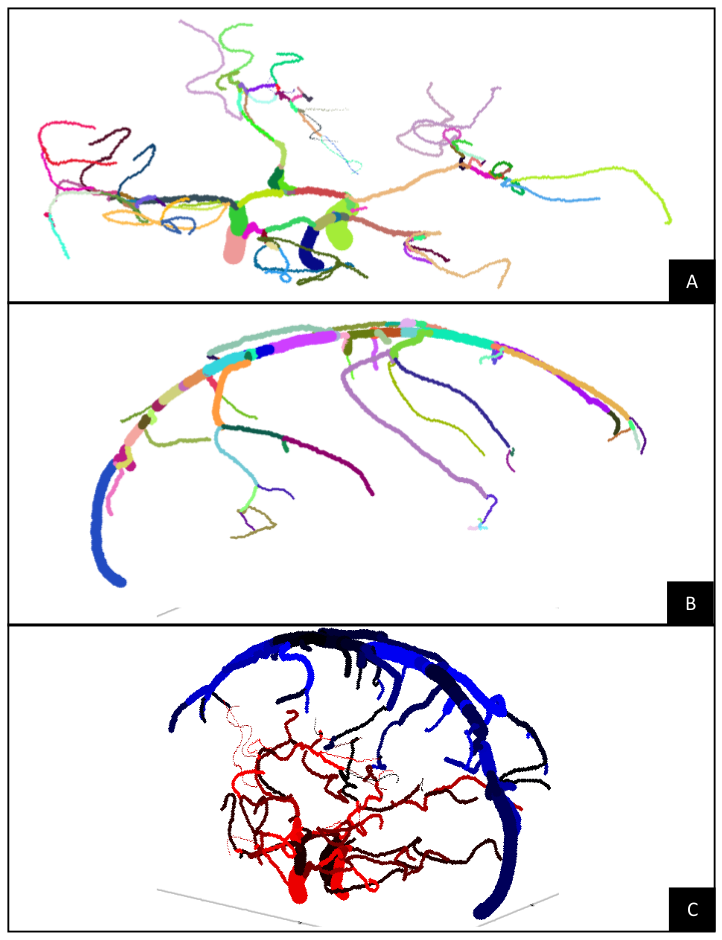
\includegraphics[width=9cm]{4_11_structure_sujet}
\caption{Architecture de référence utilisée pour évaluer la viabilité du modèle. A) L'arbre artériel, où chaque couleur
représente un segment, B) l'arbre veineux, chaque couleur représente là aussi un segment, C) la combinaison des deux, en
dégradé bleu les veines, et en rouge les artères. A noter que seuls les segments utilisés dans la simulation sont illustrés, le
« super-sinus » n’apparait pas dans cette vue. Enfin le diamètre de chaque tube est illustré par le diamètre des segments.}
\label{fig:4_11_structure_sujet}	
\end{figure}
Afin de simuler correctement le système, il est important de définir les pressions en entrée. A
partir des images en contraste de phase dynamique, nous mesurons les vitesses dans l’artère basilaire,
et les carotides internes. Ces données sont ajustées par une combinaison de fonctions trigonométrique
(Fourier, voir Figure~\ref{fig:4_12_fourier}	). On obtient ainsi 17 coefficients des séries de Fourier discrètes. Pour finir on
convertit cette cinétique en pression en plaçant le premier coefficient à une valeur de 100. Cette valeur
étant ajustée au vue des débits afin de faire correspondre les débits les plus élevés aux pressions les
plus grandes. On obtient ainsi des pressions moyennes en entrée proches de 100 mmHg. Chaque
entrée disposant d’une cinétique propre avec des pressions relatives concordantes avec les débits.\\
%%%
\begin{figure}[!b]
\centering
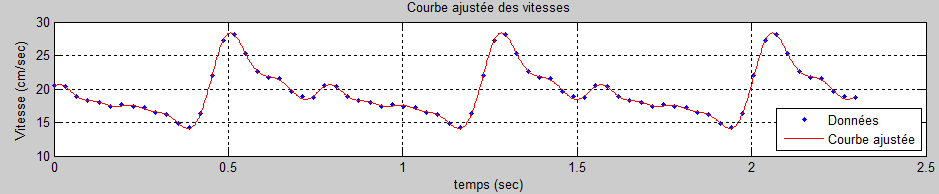
\includegraphics[width=15cm]{4_12_fourier}
\caption{Courbe ajustée des vitesses au cours du temps pour la carotide interne gauche. Ajustement par des séries de
Fourier (17 coefficients).}
\label{fig:4_12_fourier}	
\end{figure}
Les compartiments artériolaires, capillaires et veineux restent des boites noires en termes de
caractéristiques physiologiques (résistances hydrodynamiques, élastance etc.). La définition de la
résistance de ces tubes passe donc par des estimations. En vue de se rapprocher au mieux de la réalité
nous avons choisi d’utiliser les résistances utilisées par Linninger et al. (\cite{Linninger2009}) en les ajustant au vue des cartes
de perfusions ASL. Pour chaque territoire perfusionnel obtenu à partir des segmentations
morphologiques, la valeur moyenne du débit est extraite (Figure~\ref{fig:4_13_perf_ASL}, colonnes 1 et 3). Sur la base des
différences relatives entre les régions, les valeurs des résistances des artérioles, capillaires et veinules
dans chaque territoire sont ajustées (Tableau~\ref{fig:4_13_perf_ASL}). Pour les autres compartiments, les résistances sont
directement estimées à partir des informations morphologiques disponibles pour chaque segment. Les
valeurs d’élastances utilisées sont décrites dans la littérature (\cite{Zagzoule1986},~\cite{Linninger2009},~\cite{Smillie2004}) et rapportées dans le
Tableau~\ref{tab:elastances}. Les flux constants $S^{const}_{Cp\rightarrow cerv}$ et $S{const}_{cerv\rightarrow Lv}$ sont fixés à 0.0005 ml/s tandis que la
production de LCS $S_{Al\rightarrow Lv}$ est de 0.003 ml/s (\cite{Linninger2009}). Enfin la résistance utilisée pour traduire la résorptiondu LCS par le sinus veineux est de 7 $\frac{mmHg}{ ml/min}$ (valeur moyenne normale identifiée dans la littérature) (\cite{Ekstedt1978}). La viscosité du sang est établie à $\mu_{sang}$ = 0.004 $\frac{kg}{ m}$ par sec (\cite{Pedley1980}).\\
%%%
\begin{figure}[!t]
\centering
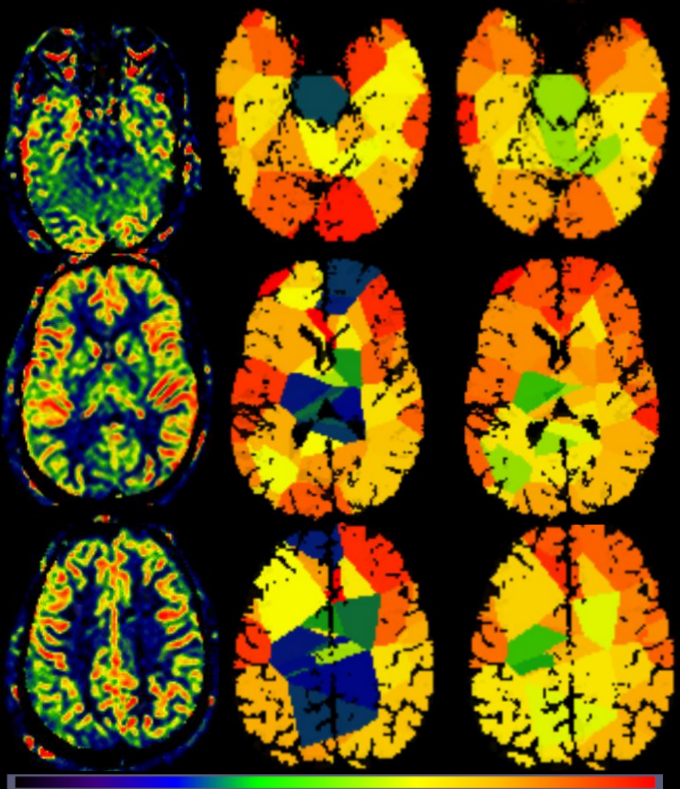
\includegraphics[width=12cm]{4_13_perf_ASL}
\caption{Perfusion cérébrale en ASL, valeurs brutes et rapportées aux différents territoires. La première colonne illustre la
carte de débit brute, la deuxième colonne la valeur relative du débit estimé par le modèle pour chaque région, et la troisième
la valeur moyenne sur la base des données ASL.}
\label{fig:4_13_perf_ASL}	
\end{figure}

\begin {table}
	\caption{Détails des élastances et résistances utilisées dans le modèle. Les résistances renseignées par un « * » sont
ajustées au vu des données ASL.} 
	\label{tab:elastances} 
	\centering
	\begin{tabularx}{\linewidth}{  X | X | X }

	{\bf Compartiment}  & { \bf \'Elastance (Pa)} & {\bf Résistance (mmHg.s.mL$^{-1}$)} \\
\hline
	{\bf Artères} & 27.3 10$^4$ (\cite{Zagzoule1986}) & {\em estimée}\\
{\bf Artérioles} & 40.0 10$^4$ (\cite{Zagzoule1986}) & 3.08$\ast$ (\cite{Linninger2009}) \\
{\bf Capillaires} & 44.0 10$^4$ (\cite{Zagzoule1986}) & 0.92$\ast$ \\
{\bf Veinuels} & 117.0 10$^4$ (\cite{Zagzoule1986}) & 0.23$\ast$ \\
{\bf Veines} & 5 10$^4$ (\cite{Zagzoule1986}) & {\em estimée}\\
{\bf Sinus} & 2.6 10$^4$ (\cite{Zagzoule1986}) & {\em estimée}\\
{\bf Ventricules} & 8.0 10$^4$ (\cite{Smillie2004}) & 1$\ast$ (\cite{Linninger2009}) \\
{\bf Espace sous arachno\"i dien} & 1.0 10$^4$ (\cite{Zagzoule1986}) & 1$\ast$ (\cite{Linninger2009}) \\
{\bf Moelle épinière} & 1.0 10$^6$ (\cite{Smillie2004}) & 0.1$\ast$ (\cite{Linninger2009}) \\
{\bf Parenchyme cérébral} & 1.0 10$^3$ (\cite{Smillie2004}) & 500-8152.42 $\ast$ (\cite{Linninger2009}) \\
	\end{tabularx}
\end{table}





Le système peut ainsi être simulé. Pour des raisons évidentes de clarté il est difficile de
représenter les résultats pour l’ensemble des compartiments sur une même figure. Nous décrirons
donc les valeurs moyennes dans chaque type de compartiments, sauf dans quelques cas précis où nous
exposerons la cinétique dans un tube particulier.\\
La pression intracrânienne identifiée par le modèle est de 9 mmHg, ce qui se situe dans la
gamme des valeurs normales chez le sujet sain (\cite{Steiner2006},~\cite{Pattinson2005}). Nous n’avons cependant pas pu la comparer
à la valeur réelle. La cascade de chute de pression des entrées aux sorties est un bon élément pour
évaluer la consistance du modèle. La pression moyenne dans les artères est de 82 mmHg, puis 49
mmHg dans les artérioles, 28 mmHg dans les capillaires et 22 et 18 mmHg respectivement dans les
veinules et veines. La comparaison de nos résultats avec les travaux précédents (Figure~\ref{fig:4_15_evolution_pression}), met en
évidence une bonne similitude entres les données de Zagzoule et Marc-Vergnes (\cite{Zagzoule1986}) à et de Linninger
et al. (\cite{Linninger2009}) . La différence majeure apparait au niveau des artérioles où notre modèle présente une chute
plus importante de la pression.\\
%%%
\begin{figure}[!t]
\centering
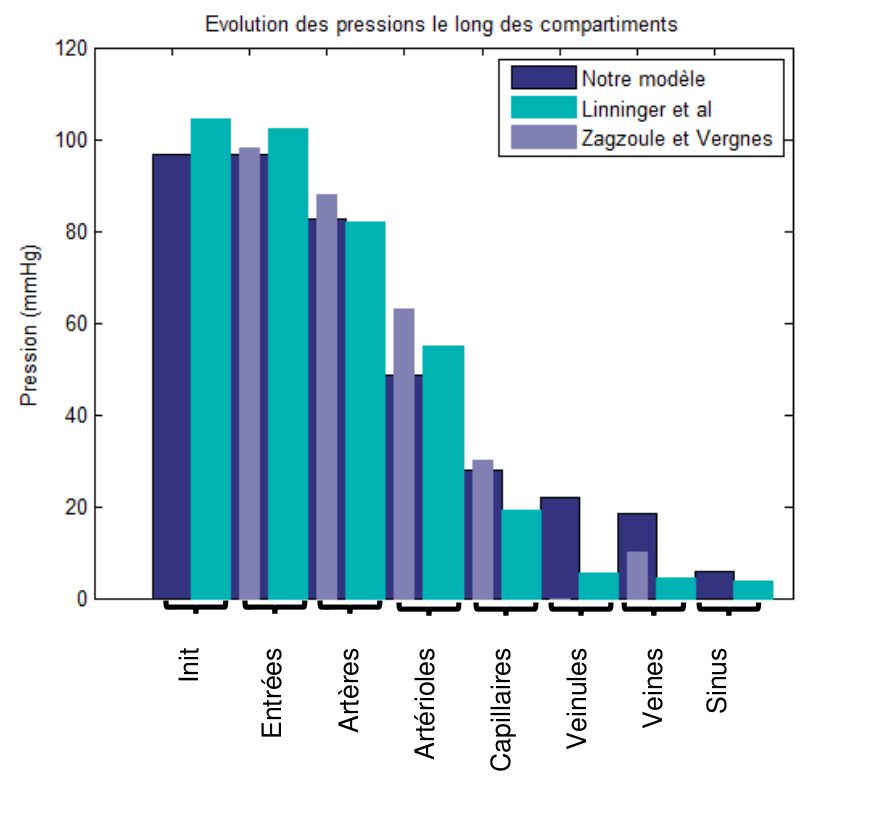
\includegraphics[width=11cm]{4_15_evolution_pression}
\caption{Evolution des pressions d'un type de compartiment à l'autre et comparaison avec les modèles similaires. Les
barres sont positionnées au vue de l’emplacement des mesures de pressions dans les différents modèles.}
\label{fig:4_15_evolution_pression}	
\end{figure}
Le détail des cinétiques de pressions au sein des différents types de compartiments (Figure~\ref{fig:4_16_decours_pression})
met en évidence la chute de pression moyenne, avec atténuation de l’amplitude au fur et à mesure
que l’on avance dans le réseau vasculaire ou ventriculaire. Les pressions moyennes dans les ventricules
évoluent elles aussi dans les gammes attendues de 7 à 10.5 mmHg (\cite{Agamanolis2011}) (Figure~\ref{fig:4_16_decours_pression} droite) avec des
cinétiques cohérentes. Le modèle prédit une pression pulsatile de 3.5 mmHg en accord avec les
données connues (3 – 5 mmHg) (\cite{Czosnyka2005}).\\
%%%
\begin{figure}[!b]
\centering
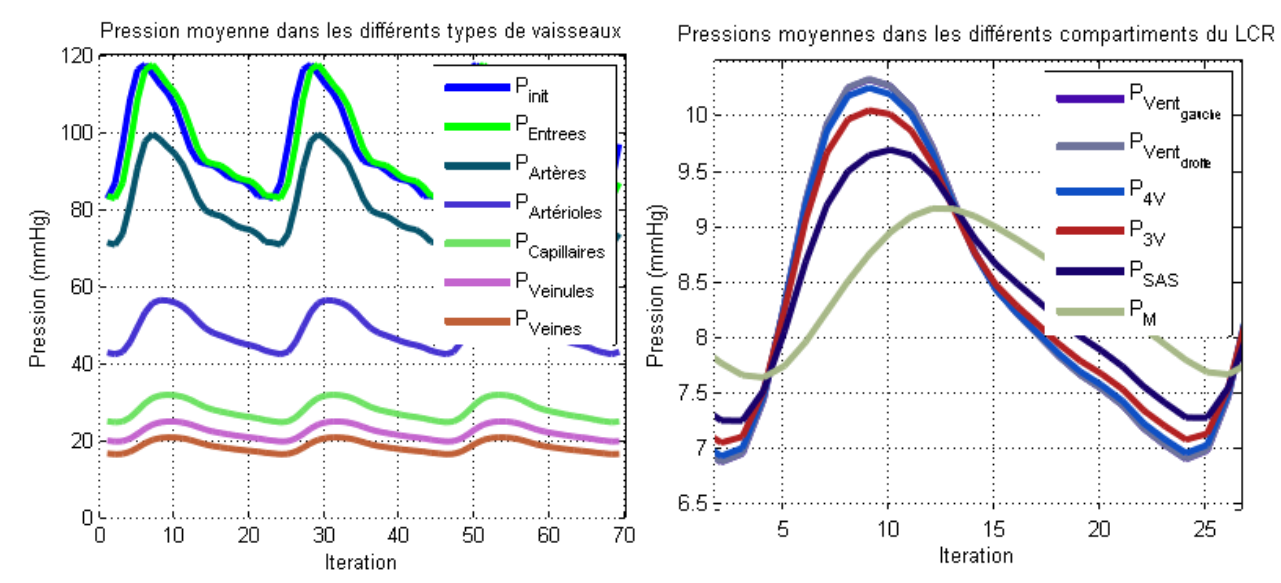
\includegraphics[width=15cm]{4_16_decours_pression}
\caption{Evolution des pressions moyennes de chaque type de compartiment. A gauche les vaisseaux, à droite les
ventricules.}
\label{fig:4_16_decours_pression}	
\end{figure}
Le débit moyen observé en entrée dans le système est de 2.45, 5.67 et 4.15 mL/sec pour
l’artère basilaire, et les carotides internes gauche et droites, soit un débit total de 12.27 mL/sec.
L’acquisition en contraste de phase dynamique nous montre que le débit est en réalité de 3, 4.49 et
4.2 mL/sec respectivement pour l’artère basilaire, la carotide interne gauche et la carotide interne
droite pour un total de 11.69 mL/sec. Malgré de faibles écarts entre les valeurs simulées et les valeurs
réelles, les données semblent cohérentes. Il est néanmoins à observer que la carotide interne gauche
présente dans le modèle un débit 20\% plus important que dans la réalité. Ce décalage devrait être
corrigé dans une version en cours de développement du modèle où les flux serviront de conditions
limites.\\
%%%
\begin{figure}[!t]
\centering
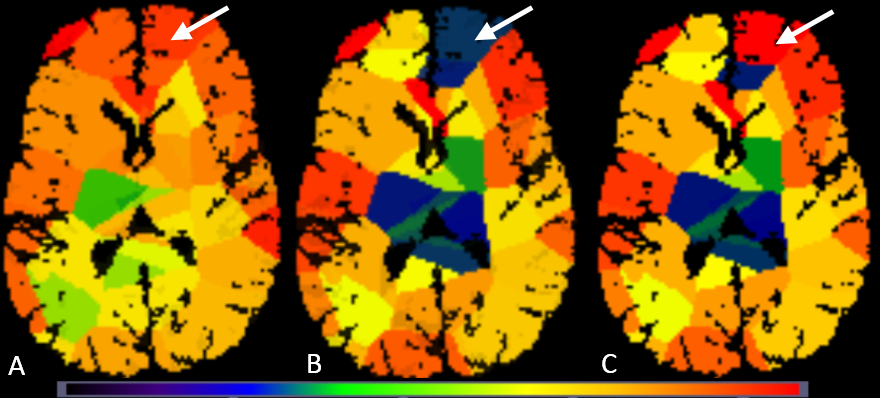
\includegraphics[width=13cm]{4_26_effet_ajout_artere_sur_cbf}
\caption{Impact de l'ajout d'une artère terminale pour un territoire. A) débit moyen par territoire mesuré en ASL, B) débit estimé par le modèle initial et C) débit estimé après ajout d'une artère parallèle. Les flèches blanches illustrent le territoire concerné. L'ajout de l'artère permet de nous rapprocher de la réalité mesurée en ASL.}
\label{fig:4_26_effet_ajout_artere_sur_cbf}	
\end{figure}
%%%
%%%
\begin{figure}[!b]
\centering
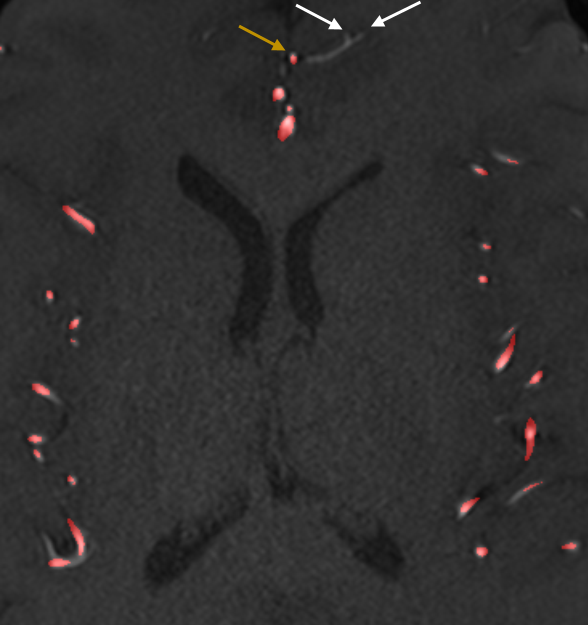
\includegraphics[width=8cm]{4_27_segmentation}
\caption{Segmentation des artères dans un territoire où l'écart entre l'ASL et le modèle est important. En rouge est représenté la segmentation. La flèche orange indique l'artère correspondante au territoire d'intérêt, les flèches blanches mettent en évidence deux autres branches associées à cette artère qui n'ont pas été segmentées.}
\label{fig:4_27_segmentation}	
\end{figure}
%%%
La Figure~\ref{fig:4_17_decours_debit} met en évidence les cinétiques observées dans les différents compartiments ; on
peut observer le décalage des cinétiques au cours de l’évolution à travers les compartiments. Le délai
artério-veineux (« phase-lag ») identifié dans le modèle est de 18 \% du cycle cardiaque, ce qui est plus
élevé que les valeurs trouvées dans la littérature (13 \%) (\cite{Linninger2009},~\cite{Kim2007}). Cette différence peut s’expliquer par
le fait que nous ne disposons pas, malgré tous nos efforts, du même niveau de détails pour les artères
et pour les veines. Les débits moyens que nous récupérons dans les compartiments artériels et veineux
reflètent en partie cette différence puisque les moyennes ne sont pas effectuées sur des niveaux
exactement comparables de l’arborescence. Les moyennes effectuées sur les veines incorporent
proportionnellement moins de petits vaisseaux que la moyenne sur les artères. L’analyse du débit
moyen dans les capillaires (Figure~\ref{fig:4_13_perf_ASL} deuxième colonne) met en évidence des différences relatives
entre les territoires en grande partie similaires aux résultats obtenus en ASL (Figure~\ref{fig:4_13_perf_ASL} troisième
colonne). Néanmoins de fortes différences existent pour certaines régions pouvant être liées à une mauvaise détection de certains vaisseaux ou à de
mauvaises associations artères – veines dans la définition structurelle du modèle. L'outil BraVa (\cite{Wright2013}, voir~\ref{sec:tubesestimates}) vu précédement, met en évidence pour notre modèle, un taux d'identification des artères de l'ordre de 55\% (voir Tableau~\ref{tab:tab_profil_rayons}). Il est probable alors que pour ces territoires, la segmentation n'ait pas permis d'obtenir le bon nombre de branches. Afin de tester cette hypothèse nous avons sélectionné un territoire pour lequel l'écart entre l'ASL et le modèle est le plus important pour simuler la présence d'un autre ensemble artère - artériole  - capillaire - veinule - veine parallèle à celui d'origine et de mêmes caractéristiques. Nous avons avons alors deux artères pour le même territoire. La Figure~\ref{fig:4_26_effet_ajout_artere_sur_cbf} illustre les résultats obtenus. L'ajout d'une branche parallèle permet d'assurer un apport supplémentaire dans le territoire concerné et ainsi de se rapprocher des données ASL. L'observation des résultats de segmentation dans cette zone (Figure~\ref{fig:4_27_segmentation}) mettent en évidence deux branches supplémentaires n'ayant pas été segmentées (flèches blanche). Cela confirme donc que l'une des sources du décalage entre le modèle et la réalité est la qualité de la segmentation.\\
%%%
\begin{figure}[!t]
\centering
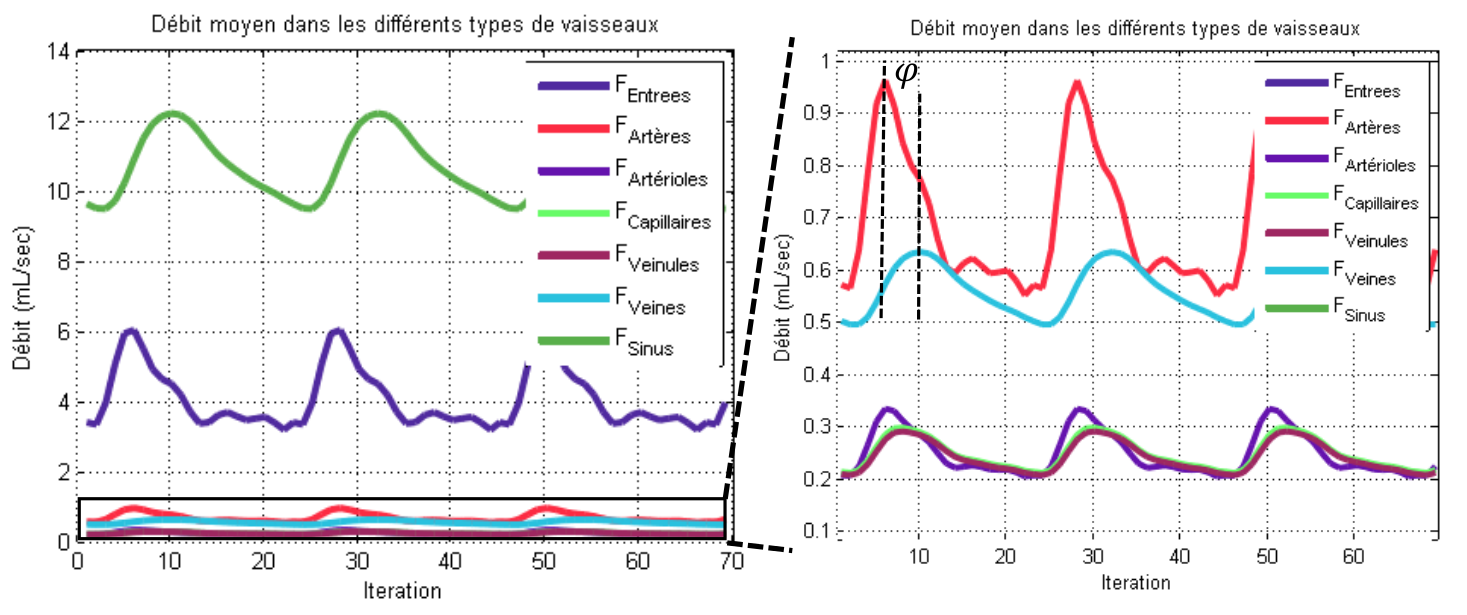
\includegraphics[width=15cm]{4_17_decours_debit}
\caption{Evolution des débits moyens dans les compartiments vasculaires. Sur l’image de droite, en pointillés noir, est
renseigné le délai artério-veineux $\phi$.}
\label{fig:4_17_decours_debit}	
\end{figure}
Les débits dans les compartiments ventriculaires sont illustrés dans la Figure~\ref{fig:4_19_debit_ventriculaire}. Les mesures
réalisées en contraste de phase au niveau de l’aqueduc estiment le débit à 0.011 mL/sec avec une
amplitude de 0.32 mL/sec. Notre modèle prévoit dans cette zone un débit moyen de 0.009 mL/sec
avec une amplitude de 0.33 mL/sec. Le modèle est donc en bon accord avec les données disponibles.
Enfin l’évolution de l’aire est elle aussi gérée par le modèle et est cohérente avec l’évolution des
pressions (Figure~\ref{fig:4_20_aire_artere}), quoi que plus difficile à valider expérimentalement compte tenu de la résolution.\\
%%%
\begin{figure}[!b]
\centering
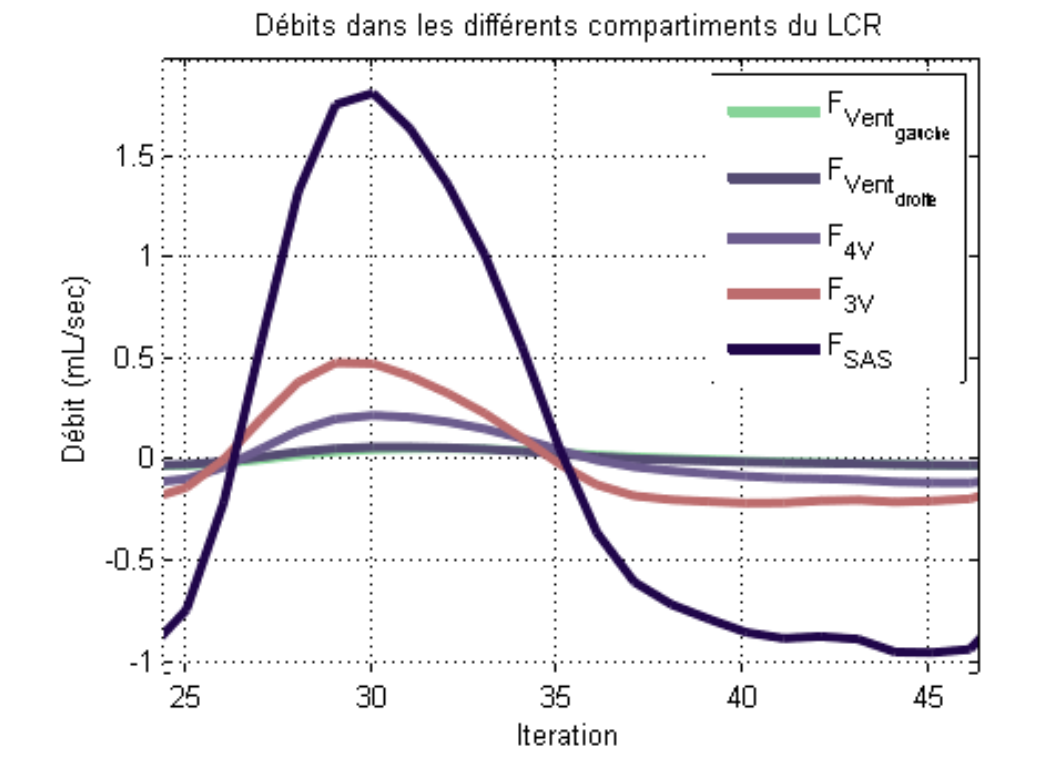
\includegraphics[width=10cm]{4_19_debit_ventriculaire}
\caption{Estimation par le modèle des débits dans les compartiments ventriculaires.}
\label{fig:4_19_debit_ventriculaire}	
\end{figure}
%%%
\begin{figure}[!t]
\centering
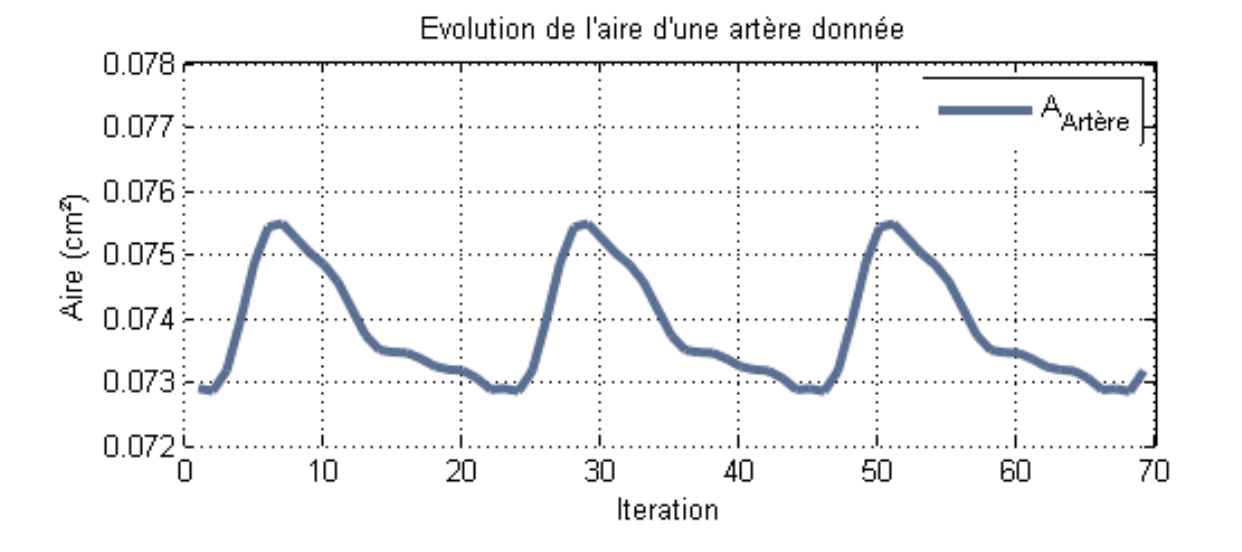
\includegraphics[width=15cm]{4_20_aire_artere}
\caption{Evolution de l'aire d'une artère donnée au cours du temps estimée par le modèle.}
\label{fig:4_20_aire_artere}	
\end{figure}
En vue d’exploiter plus en détail notre modèle complet sujet-spécifique, nous avons réalisé des
simulations en augmentant artificiellement la résistance d’une artère afin d’évaluer l’évolution des flux
dans les artères en aval et d’observer ainsi la compensation offerte par les artères communicantes. En
l’absence de cette occlusion, notre modèle prédit logiquement des débits plus importants au niveau
des entrées puis une chute jusqu’aux capillaires. Les veines récupèrent ensuite le sang et l’acheminent
vers le sinus veineux ce qui se traduit par une augmentation du débit. Les artères communicantes
(postérieure gauche et antérieure) présentent des débits très faible (violet foncé) (Figure\ref{fig:4_21_debit_moyen}).\\
%%%
\begin{figure}[!b]
\centering
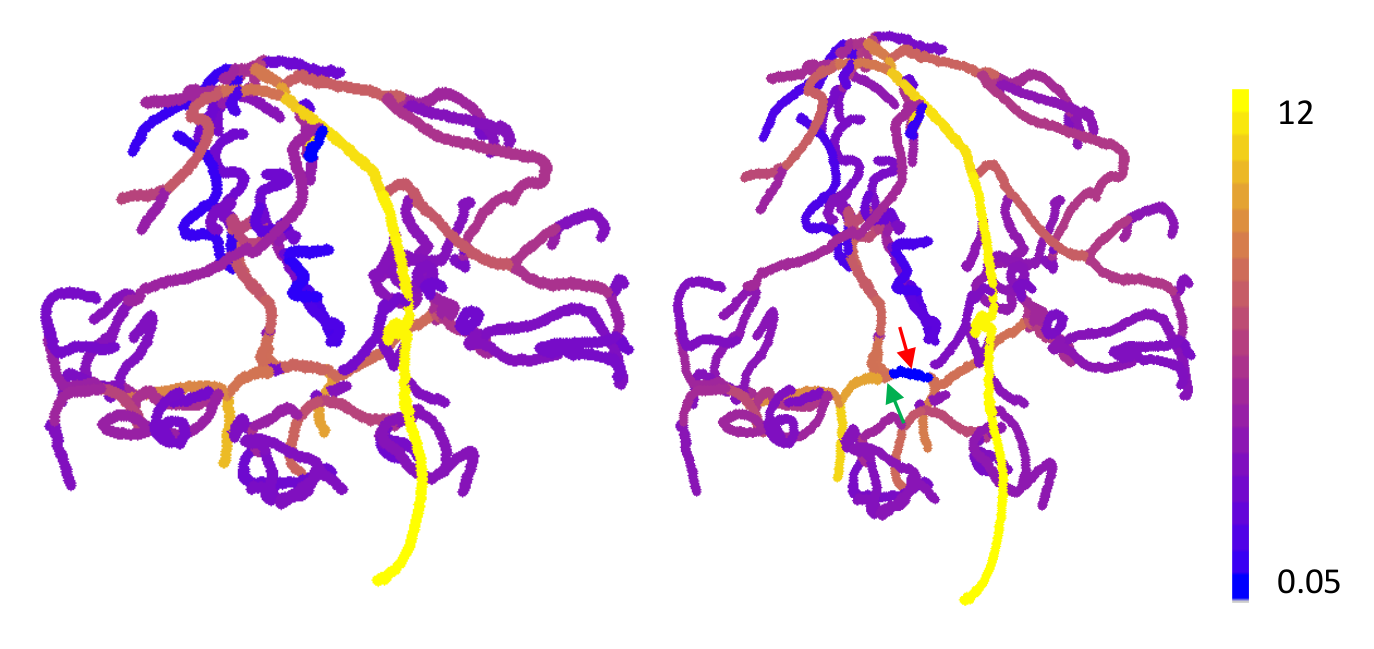
\includegraphics[width=15cm]{4_21_debit_moyen}
\caption{Débits moyens dans les différentes artères et veines du modèle. A gauche la répartition pour le modèle initial du
sujet, à droite la répartition après avoir augmenté artificiellement la résistance d’un segment de l’artère cérébrale
antérieure (flèche rouge). La flèche verte indique l’emplacement de l’artère communicante antérieure (ACoA). Une échelle
de couleur logarithmique est utilisée.}
\label{fig:4_21_debit_moyen}	
\end{figure}
Si l’on augmente alors fortement la résistance d’un tube (début de l’artère cérébrale
antérieure) de manière à simuler une occlusion (Figure\ref{fig:4_21_debit_moyen} flèche rouge), on peut observer l’utilisation
de la voie de compensation que représente l’artère communicante antérieure (ACoA) (flèche verte).
Le détail de cette compensation est illustré en Figure~\ref{fig:4_22_flux_ACA} A. Comme on peut le voir, chez ce sujet l’ACoA
est efficace puisqu’elle permet d’assurer un apport quasi-normal en sang dans l’ACA même lorsque sa
partie amont est occluse. Ce sujet présente une ACoA de bon diamètre (2.3 mm) pouvant être définie
comme « normale » selon Tulleken (\cite{Tulleken1978}). Des études ont montré que le diamètre moyen de cette
artère se situait entre 1.5 (\cite{Perlmutter1976}) et 1.92±0.86 mm (\cite{Hillen1986}). Cassot et al. (\cite{Cassot1995}) ont évalué l’effet du diamètre
de l’ACoA lors de sténoses carotidiennes. Via un modèle dédié au polygone de Willis, ils ont pu simuler
l’évolution des flux et des pressions en fonction du degré de sténose et du diamètre de l’ACoA. Leurs
résultats montrent tout d’abord une augmentation du débit dans la carotide controlatérale à l’artère
occluse de 73.7 \% avec 47.3 \% du débit total de l’artère dédiée à l’ACoA. Dans notre simulation, la
carotide interne n’est pas bouchée, c’est le premier segment de l’ACA qui l’est. Nous ne mettons en
évidence qu’une augmentation de 26 \% avec 25 \% du débit total de la carotide controlatérale dédiée
à l’ACoA. Si nous simulons des conditions similaires à celles de Cassot et al. nous mettons en évidence
une augmentation de 65 \% avec 43 \% dédiée à l’ACoA, les résultats semblent donc concordants malgré
une augmentation plus faible du débit pouvant être expliquée par l’absence (chez notre sujet) d’artère
communicante postérieure droite.\\
%%%
\begin{figure}[!t]
\centering
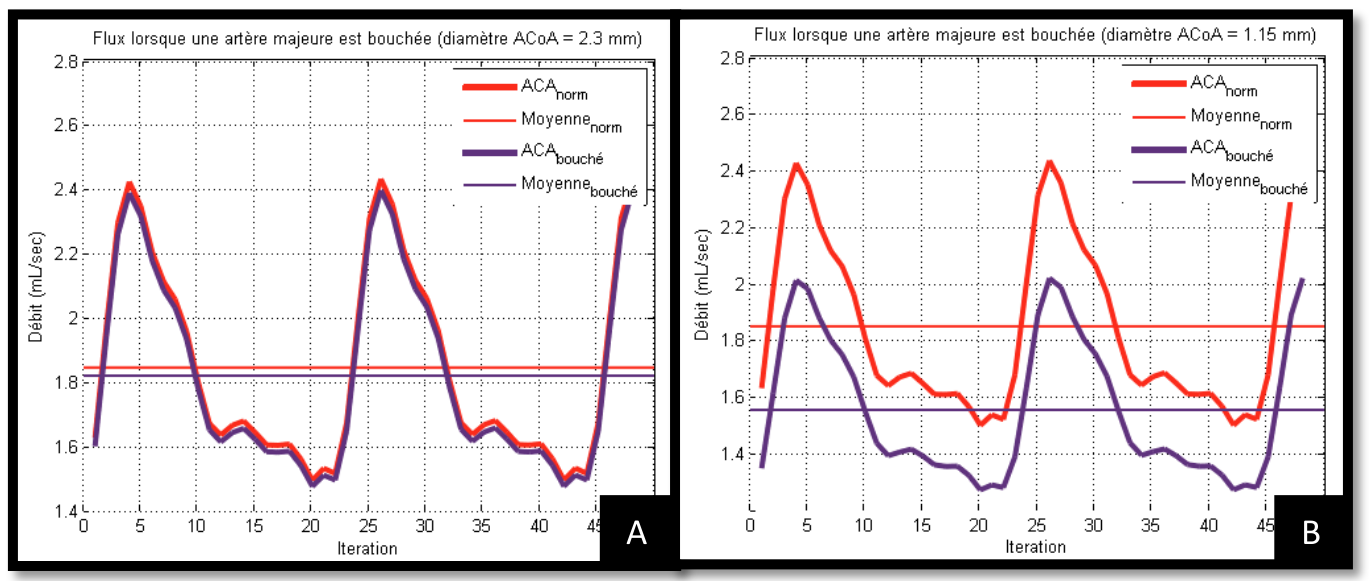
\includegraphics[width=15cm]{4_22_flux_ACA}
\caption{ Flux dans l'artère cérébrale antérieure (ACA) droite après augmentation de la résistance de sa partie amont. A)
flux dans le modèle initial, avec artère communicante antérieure (ACoA) de diamètre 2.3 mm (valeur réelle). B) En réduisant
artificiellement le diamètre de l’ACoA à 1.15 (facteur 2). L’ACoA assure un maintien suffisant du débit dans l’ACoA dans la
version initiale, ce maintien diminue avec la réduction du calibre de l’ACoA. L’indice « norm » indique la situation normale, et
« bouché » la situation lorsque le premier segment de l’ACA est occlus.}
\label{fig:4_22_flux_ACA}	
\end{figure}
Dans notre simulation le premier segment de l’ACA droite du sujet est occlus. Pour évaluer la
capacité de compensation de l’ACoA sur le flux dans ces conditions nous avons fait varier son diamètre
de façon similaire aux travaux de Cassot et al. (\cite{Cassot1995}). La compensation de l’ACoA est analysée en faisant
le rapport entre le débit dans le segment en aval de l’ACoA après occlusion et avant l’occlusion,
donnant un indice en pourcentage. Les résultats illustrés en Figures~\ref{fig:4_23_compensation_ACoA},~\ref{fig:4_24_occlusion_ventricule}, et~\ref{fig:4_25_impact_occlusion} montrent aux vue de l’intervalle
de variation de la sigmoïde1, une évolution importante de la compensation dans la gamme de diamètre
allant de 0.37 à 1.17 mm. Les valeurs inférieures ne permettent pas une compensation efficace, et les
valeurs plus élevées permettent d’assurer près de 90\% du débit de l’artère occluse. La limite supérieure
de cette zone est plus faible que celle rapportée précédemment (0.4 à 1.6 mm,~\cite{Cassot1995}). Néanmoins, il est
important de rappeler que notre modèle est spécifiquement adapté à un sujet donné ce qui peut
expliquer les écarts de ce type.\\
%%%
\begin{figure}[!t]
\centering
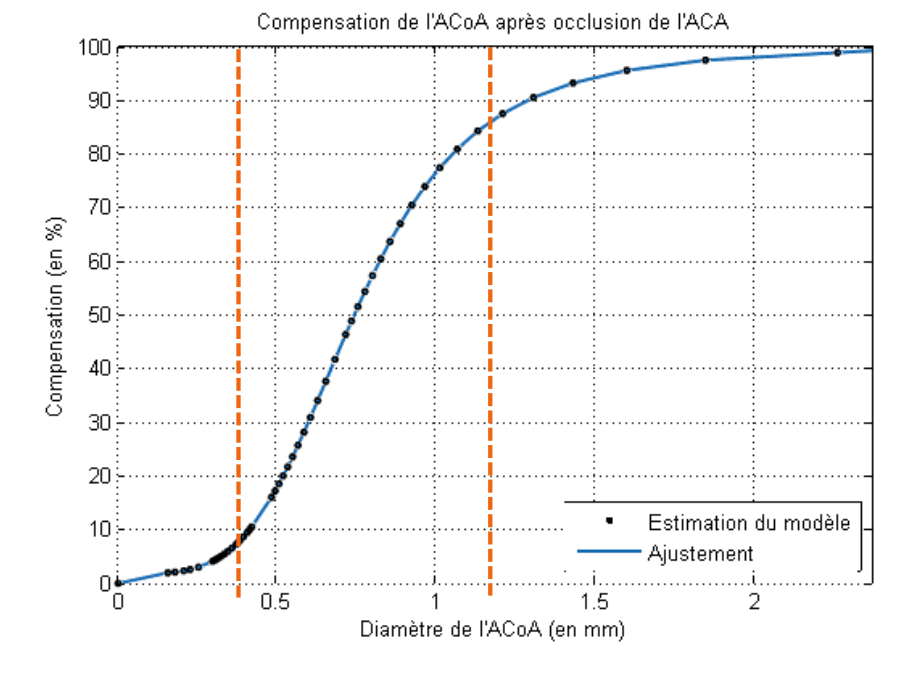
\includegraphics[width=11cm]{4_23_compensation_ACoA}
\caption{ Degré de compensation de l'ACoA lors de l'occlusion du premier segment de l'ACA droite en fonction du diamètre
de l'ACoA. La compensation est représentée comme le rapport entre le débit dans le segment en aval de l’ACoA après
occlusion et avant l’occlusion. Les lignes en pointillées orange indiquent l’intervalle de variation de la sigmoïde
respectivement 0.37 et 1.17 mm. Cette zone correspond aux plus fortes variations de compensation en fonction du diamètre
de l’ACoA.}
\label{fig:4_23_compensation_ACoA}	
\end{figure}
L’avantage de notre méthodologie est qu’elle intègre l’ensemble des flux intracrâniens, y
compris le liquide cérébro-spinal. Il est donc possible de mettre en évidence l’impact de l’occlusion sur
ces compartiments. La Figure~\ref{fig:4_19_debit_ventriculaire} dédiée aux ventricules latéraux, montre une chute des débits entrant
dans les deux hémisphères lorsque le diamètre de l’ACoA diminue. La chute dans le ventricule
controlatéral à l’occlusion peut être vu comme un reflet de la chute globale du débit dans l’ensemble
du système. Du côté ipsilatéral, la diminution est plus marquée du fait de la diminution de l’apport
sanguin dans certains territoires et donc des flux capillaires/parenchyme puis parenchyme/ventricules.
De la même façon l’aire augmente de façon plus importante du côté ipsilatéral sans doute par réaction
mécanique. Notons que malgré des évolutions faibles (moins de 2 \%), le modèle est suffisamment
sensible pour les mettre en évidence.\\
%%%
\begin{figure}[!t]
\centering
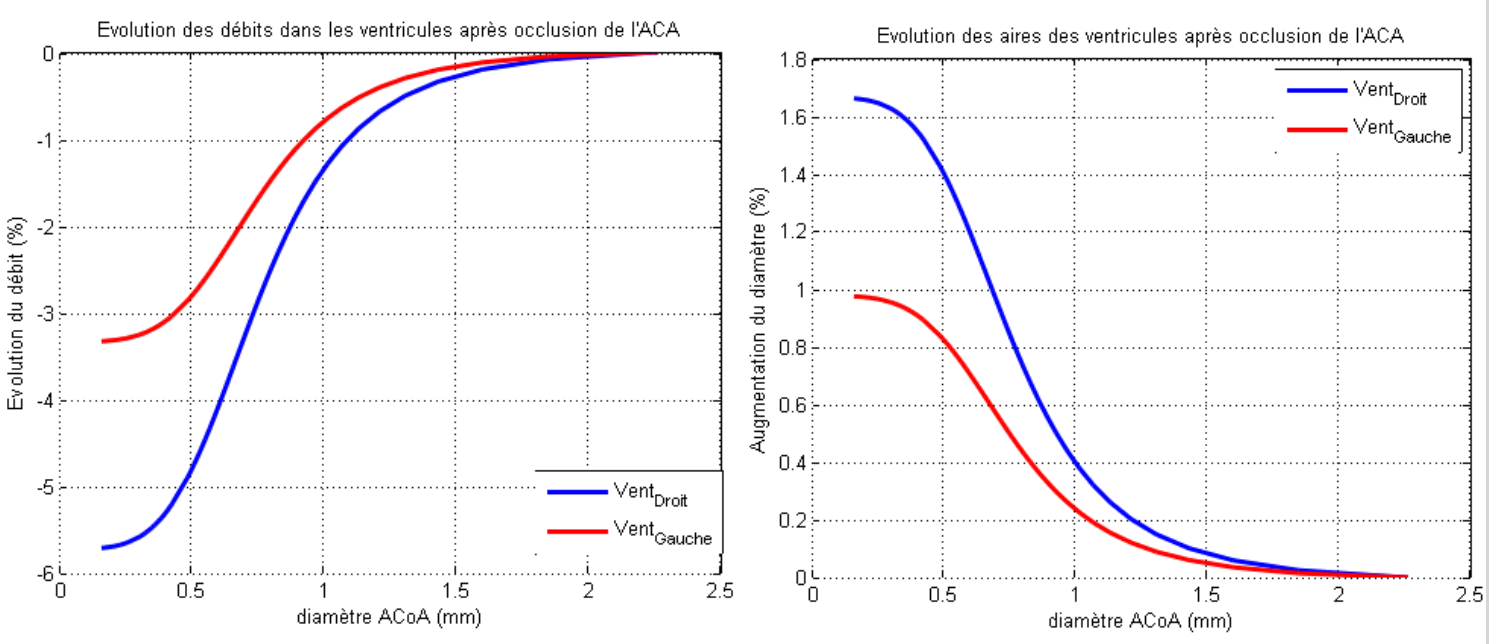
\includegraphics[width=15cm]{4_24_ventricules_occlusion}
\caption{ Evolution des débits entrants et des aires des ventricules en réponse à une occlusion de l'ACA droite. Les données
sont représentées en fonction du diamètre de l'ACoA. A gauche l’évolution du débit entrant (en \%). On remarque en rouge
une chute du débit entrant dans le ventricule droit en fonction de la diminution de diamètre de l’ACoA (3.3 \%). Il s’agit du
reflet de l’effet global sur les débits de l’occlusion. La chute est plus marquée dans le ventricule droit ipsilatéral à l’occlusion
(5.75 \%). Le graphique de droite illustre l’évolution relative de l’aire des ventricules en fonction du diamètre de l’ACoA.
Comme pour les débits on observe un effet plus important du côté ipsilatéral à l’occlusion, malgré tout l’évolution reste très
faible (1.7 \%).}
\label{fig:4_24_occlusion_ventricule}	
\end{figure}
Par ailleurs, le modèle offre l’opportunité de localiser les effets au niveau capillaire au vu des
territoires définis (Figure~\ref{fig:4_13_perf_ASL} et Figure~\ref{fig:4_25_impact_occlusion}). En plus d’une chute globale relativement faible du débit
dans l’ensemble des territoires, on observe à partir d’un diamètre de l’ACoA divisé par deux une chute
marquée du débit dans les territoires de l’ACA, avec la présence d’inhomogénéités dans cette zone
traduisant des effets différents selon la région.\\
%%%
\begin{figure}[!t]
\centering
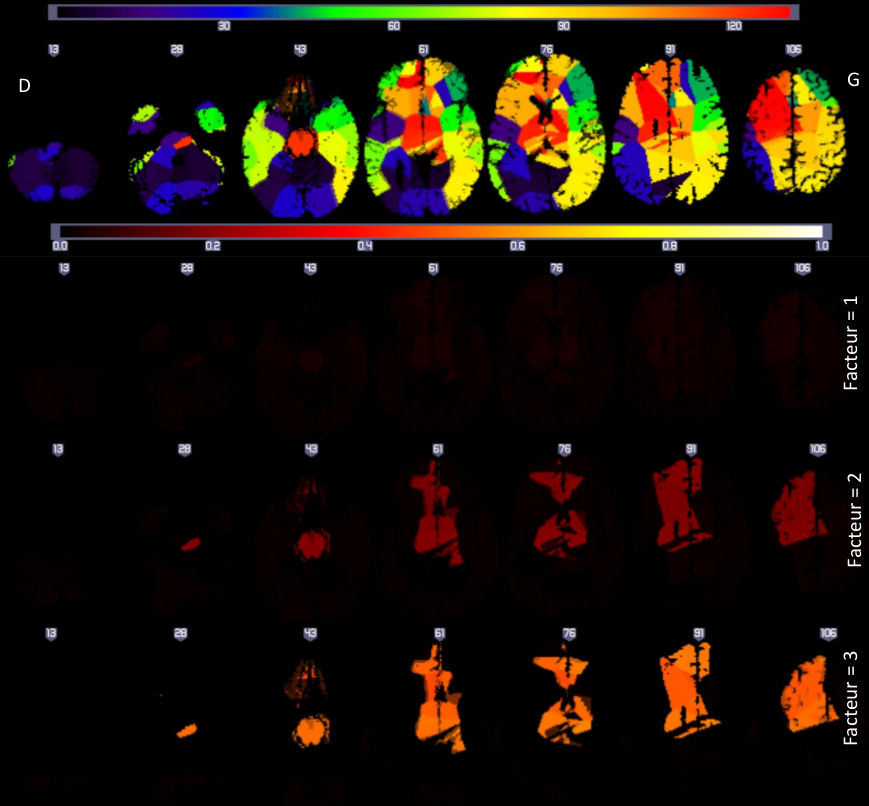
\includegraphics[width=15cm]{4_25_impact_occlusion}
\caption{ Impact de l'occlusion du premier segment de l'ACA droite selon différents diamètres de l'ACoA. La première ligne
illustre les territoires définis, les seconde, troisième et quatrième lignes illustrent le degré de réduction du débit (de 0 à 1)
dans ces territoires avec le diamètre original de l’ACoA (facteur = 1, 2.3 mm), divisé par deux (facteur = 2, 1.15 mm), et divisé
par 3 (facteur = 3, 0.77 mm).}
\label{fig:4_25_impact_occlusion}	
\end{figure}
Pour conclure cette partie, on peut donc dire que 1) notre modèle montre ainsi sa cohérence
avec les modèles existants dédiés à certaines structures (\cite{Cebral2003},~\cite{Cassot1995}), ou représentant l’ensemble du
système en simplifiant le problème (\cite{Zagzoule1986},~\cite{Linninger2009},~\cite{Kim2007}). Par ailleurs 2) il est également compatible avec les
données disponibles mesurées en IRM. Du fait de son caractère sujet-spécifique, il autorise de plus
l’investigation de nombreuses problématiques supplémentaires, ce qui sera l’objet des travaux
ultérieurs.


\bibliography{jeremythesebib}{}
\bibliographystyle{francaissc}